\documentclass[informe.tex]{subfiles}
\begin{document}
  
  \section{Resultados}
    Para analizar los distintos métodos decidimos generar 9 folds con los datos. Teniendo un conjunto provisto es de 900 datos, cada entrenamiento se realiz\'o con 800 entradas y la validación con las 100 restantes. Además, cada experimento fue repetido 5 veces a fin de tener diferentes corridas de cada caso y observar si se produc\'ian diferentes resultados con cada una.
    
    \subsection{Reducción de dimensiones}
      Para analizar este modelo se consideraron los dos criterios de parada mencionados anteriormente: componentes principales ortogonales y $\Delta W$ nulo. Para cada una de esas opciones se usaron las reglas de Oja y de Sanger de modo de poder probar las distintas combinaciones y comparar sus resultados. 
      
      ~
      
      En cada experimento se realizó un gráfico en el cual cada instancia se indica en un espacio tridimensional correspondiente a las tres componentes principales con diferentes colores según la clase. Allí, cada clase de entre las posibles (1 al 9) recibe un color y las instancias de entrenamiento son representadas con un círculo mientras que las de validación se indican con un triángulo. El objetivo entonces es observar cuál es la distribución de las instancias en ese espacio.
      
      ~
      
      El l\'imite de cantidad de \'epocas elegido fue $500$ considerando que es un n\'umero lo suficientemente grande para que el método converja. En todos los casos, si no se llega a que los vectores sean ortogonales o bien que $\Delta W$ sea pequeño entonces el criterio de corte es alcanzar ese límite máximo de épocas. Además, el valor de epsilon elegido fue $0.001$.

      \subsubsection{Resumen de resultados}
      
	En todos los casos 
	\begin{itemize}
	\item $A$ es ``Cantidad de veces con corte por máximo de épocas''
	\item $B$ es ``Cantidad de veces con corte por ortogonalidad''
	\item $C$ es ``Corte por épocas error mínimo''
	\item $D$ es ``Corte por épocas error máximo''
	\item $E$ es ``Corte por épocas error promedio''
	\item $F$ es ``Corte por ortogonalidad cantidad de épocas mínima''
	\item $G$ es ``Corte por ortogonalidad cantidad de épocas máxima''
	\item $H$ es ``Corte por ortogonalidad cantidad de épocas promedio''
	\end{itemize}
  
	
	\myparagraph{Usando 500 épocas como máximo}
	\begin{table}[H]
	  \centering
	  \begin{tabular}{|l|l|l|l|l|l|l|l|l|} \hline
	  Fold & $A$ & $B$ & $C$ & $D$ & $E$ & $F$ & $G$ & $H$ \\ \hline
	  1& 4 & 1 & 0.004782 & 0.004782 & 0.004782 & 18 & 18 & 18 \\ \hline
	  2& 4 & 1 & 0.004761 & 0.004761 & 0.004761 & 17 & 17 & 17 \\ \hline
	  3& 4 & 1 & 0.004757 & 0.004757 & 0.004757 & 15 & 15 & 15 \\ \hline
	  4& 5 & 0 & 0.003081 & 0.003081 & 0.003081 & -- & -- & -- \\ \hline
	  5& 2 & 3 & 0.004759 & 0.004759 & 0.004759 & 11 & 17 & 14.33 \\ \hline
	  6& 4 & 1 & 0.004767 & 0.004767 & 0.004767 & 17 & 17 & 17 \\ \hline
	  7& 4 & 1 & 0.004805 & 0.004805 & 0.004805 & 13 & 13 & 13 \\ \hline
	  8& 3 & 2 & 0.004777 & 0.004777 & 0.004777 & 17 & 27 & 22 \\ \hline
	  9& 4 & 1 & 0.004733 & 0.004733 & 0.004733 & 5 & 5 & 5 \\ \hline
	  \end{tabular}
	  \caption{Resultados para los 9 folds, usando ortogonalidad como criterio de parada y usando la regla de Sanger. Las cantidades y promedios son sobre todas las repeticiones hechas.}
	  \label{tab:ortogonalidad_sanger500}
	\end{table}

	
	\begin{table}[H]
	  \centering
	  \begin{tabular}{|l|l|l|l|l|l|l|l|l|} \hline
	  Fold & $A$ & $B$ & $C$ & $D$ & $E$ & $F$ & $G$ & $H$ \\ \hline
	  1& 0 & 5 & -- & -- & -- & 22 & 27 & 23,6 \\ \hline
	  2& 0 & 5 & -- & -- & -- & 20 & 30 & 26 \\ \hline
	  3& 0 & 5 & -- & -- & -- & 23 & 31 & 25,6 \\ \hline
	  4& 0 & 5 & -- & -- & -- & 10 & 30 & 21,4 \\ \hline
	  5& 0 & 5 & -- & -- & -- & 18 & 27 & 22,8 \\ \hline
	  6& 0 & 5 & -- & -- & -- & 21 & 27 & 23 \\ \hline
	  7& 0 & 5 & -- & -- & -- & 13 & 27 & 20,4 \\ \hline
	  8& 1 & 4 & 0.004718 & 0.004718 & 0.004718 & 22 & 30 & 25,5 \\ \hline
	  9& 0 & 5 & -- & -- & -- & 1 & 25 & 17,4 \\ \hline
	  \end{tabular}
	  \caption{Resultados para los 9 folds, usando ortogonalidad como criterio de parada y usando la regla de Oja. Las cantidades y promedios son sobre todas las repeticiones hechas.}
	  \label{tab:ortogonalidad_oja500}
	\end{table}

	
	\begin{table}[H]
	  \centering
	  \begin{tabular}{|l|l|l|l|l|l|l|l|l|} \hline
	  Fold & $A$ & $B$ & $C$ & $D$ & $E$ & $F$ & $G$ & $H$ \\ \hline
	  1& 5 & 0 & 0.004782 & 0.004782 & 0.004782 & -- & -- & -- \\ \hline
	  2& 5 & 0 & 0.004761 & 0.004761 & 0.004761 & -- & -- & -- \\ \hline
	  3& 5 & 0 & 0.004757 & 0.004757 & 0.004757 & -- & -- & -- \\ \hline
	  4& 5 & 0 & 0.004767 & 0.004767 & 0.004767 & -- & -- & -- \\ \hline
	  5& 5 & 0 & 0.004759 & 0.004759 & 0.004759 & -- & -- & -- \\ \hline
	  6& 5 & 0 & 0.004767 & 0.004767 & 0.004767 & -- & -- & -- \\ \hline
	  7& 5 & 0 & 0.004805 & 0.004805 & 0.004805 & -- & -- & -- \\ \hline
	  8& 5 & 0 & 0.004777 & 0.004777 & 0.004777 & -- & -- & -- \\ \hline
	  9& 5 & 0 & 0.004733 & 0.004733 & 0.004733 & -- & -- & -- \\ \hline
	  \end{tabular}
	  \caption{Resultados para los 9 folds, usando $\Delta W$ como criterio de parada y usando la regla de Sanger. Las cantidades y promedios son sobre todas las repeticiones hechas.}
	  \label{tab:pesos_sanger500}
	\end{table}      
	

	\begin{table}[H]
	  \centering
	  \begin{tabular}{|l|l|l|l|l|l|l|l|l|} \hline
	  Fold & $A$ & $B$ & $C$ & $D$ & $E$ & $F$ & $G$ & $H$ \\ \hline
	  1& 5 & 0 & 0.004730 & 0.004730 & 0.004730 & -- & -- & -- \\ \hline
	  2& 5 & 0 & 0.004724 & 0.004724 & 0.004724 & -- & -- & -- \\ \hline
	  3& 5 & 0 & 0.004712 & 0.004712 & 0.004712 & -- & -- & -- \\ \hline
	  4& 5 & 0 & 0.002974 & 0.002974 & 0.002974 & -- & -- & -- \\ \hline
	  5& 5 & 0 & 0.004703 & 0.004703 & 0.004703 & -- & -- & -- \\ \hline
	  6& 5 & 0 & 0.004718 & 0.004718 & 0.004718 & -- & -- & -- \\ \hline
	  7& 5 & 0 & 0.004750 & 0.004750 & 0.004750 & -- & -- & -- \\ \hline
	  8& 5 & 0 & 0.004718 & 0.004718 & 0.004718 & -- & -- & -- \\ \hline
	  9& 5 & 0 & 0.004699 & 0.004699 & 0.004699 & -- & -- & -- \\ \hline
	  \end{tabular}
	  \caption{Resultados para los 9 folds, usando $\Delta W$ como criterio de parada y usando la regla de Oja. Las cantidades y promedios son sobre todas las repeticiones hechas.}
	  \label{tab:pesos_oja500}
	\end{table}            

	
	
	
	
	Dado que en muchos de los casos el corte se produjo por alcanzarse el máximo de épocas y que las distintas repeticiones produjeron un error idéntico, decidimos repetir la experimentación pero ahora con una cantidad de épocas máxima igual a 250 para ver si de esa manera se convergía a los mismos errores pero con una menor cantidad de épocas.
	
	
	\myparagraph{Usando 250 épocas como máximo}
	\begin{table}[H]
	  \centering
	  \begin{tabular}{|l|l|l|l|l|l|l|l|l|} \hline
	  Fold & $A$ & $B$ & $C$ & $D$ & $E$ & $F$ & $G$ & $H$ \\ \hline
	  1& 5 & 0 & 0.004782 & 0.004782 & 0.004782 & -- & -- & -- \\ \hline
	  2& 2 & 3 & 0.004761 & 0.004761 & 0.004761 & 13 & 21 & 16 \\ \hline
	  3& 4 & 1 & 0.004757 & 0.004757 & 0.004757 & 16 & 16 & 16 \\ \hline
	  4& 5 & 0 & 0.003081 & 0.003081 & 0.003081 & -- & -- & -- \\ \hline
	  5& 3 & 2 & 0.004759 & 0.004759 & 0.004759 & 14 & 18 & 16 \\ \hline
	  6& 4 & 1 & 0.004767 & 0.004767 & 0.004767 & 18 & 18 & 18 \\ \hline
	  7& 4 & 1 & 0.004805 & 0.004805 & 0.004805 & 19 & 19 & 19 \\ \hline
	  8& 4 & 1 & 0.004777 & 0.004777 & 0.004777 & 12 & 12 & 12 \\ \hline
	  9& 5 & 0 & 0.004733 & 0.004733 & 0.004733 & -- & -- & -- \\ \hline
	  \end{tabular}
	  \caption{Resultados para los 9 folds, usando ortogonalidad como criterio de parada y usando la regla de Sanger. Las cantidades y promedios son sobre todas las repeticiones hechas.}
	  \label{tab:ortogonalidad_sanger250}
	\end{table}

	
	\begin{table}[H]
	  \centering
	  \begin{tabular}{|l|l|l|l|l|l|l|l|l|} \hline
	  Fold & $A$ & $B$ & $C$ & $D$ & $E$ & $F$ & $G$ & $H$ \\ \hline
	  1& 0 & 5 & -- & -- & -- & 19 & 26 & 23,2 \\ \hline
	  2& 0 & 5 & -- & -- & -- & 21 & 30 & 24 \\ \hline
	  3& 0 & 5 & -- & -- & -- & 16 & 26 & 22 \\ \hline
	  4& 0 & 5 & -- & -- & -- & 19 & 29 & 24,6 \\ \hline
	  5& 0 & 5 & -- & -- & -- & 14 & 27 & 21,8 \\ \hline
	  6& 0 & 5 & -- & -- & -- & 19 & 25 & 22,6 \\ \hline
	  7& 0 & 5 & -- & -- & -- & 18 & 34 & 25,6 \\ \hline
	  8& 0 & 5 & -- & -- & -- & 22 & 28 & 24,8 \\ \hline
	  9& 0 & 5 & -- & -- & -- & 22 & 29 & 24,8 \\ \hline
	  \end{tabular}
	  \caption{Resultados para los 9 folds, usando ortogonalidad como criterio de parada y usando la regla de Oja. Las cantidades y promedios son sobre todas las repeticiones hechas.}
	  \label{tab:ortogonalidad_oja250}
	\end{table}

	
	\begin{table}[H]
	  \centering
	  \begin{tabular}{|l|l|l|l|l|l|l|l|l|} \hline
	  Fold & $A$ & $B$ & $C$ & $D$ & $E$ & $F$ & $G$ & $H$ \\ \hline
	  1& 5 & 0 & 0.004761 & 0.004782 & 0.0047778 & -- & -- & -- \\ \hline
	  2& 5 & 0 & 0.004757 & 0.004761 & 0.0047606 & -- & -- & -- \\ \hline
	  3& 5 & 0 & 0.004757 & 0.004757 & 0.004757 & -- & -- & -- \\ \hline
	  4& 5 & 0 & 0.003081 & 0.003081 & 0.003081 & -- & -- & -- \\ \hline
	  5& 5 & 0 & 0.004759 & 0.004759 & 0.004759 & -- & -- & -- \\ \hline
	  6& 5 & 0 & 0.004767 & 0.004767 & 0.004767 & -- & -- & -- \\ \hline
	  7& 5 & 0 & 0.004805 & 0.004805 & 0.004805 & -- & -- & -- \\ \hline
	  8& 5 & 0 & 0.004777 & 0.004777 & 0.004777 & -- & -- & -- \\ \hline
	  9& 5 & 0 & 0.004733 & 0.004733 & 0.004733 & -- & -- & -- \\ \hline
	  \end{tabular}
	  \caption{Resultados para los 9 folds, usando $\Delta W$ como criterio de parada y usando la regla de Sanger. Las cantidades y promedios son sobre todas las repeticiones hechas.}
	  \label{tab:pesos_sanger250}
	\end{table}      
	

	\begin{table}[H]
	  \centering
	  \begin{tabular}{|l|l|l|l|l|l|l|l|l|} \hline
	  Fold & $A$ & $B$ & $C$ & $D$ & $E$ & $F$ & $G$ & $H$ \\ \hline
	  1& 5 & 0 & 0.004730 & 0.004730 & 0.004730 & -- & -- & -- \\ \hline
	  2& 5 & 0 & 0.004724 & 0.004724 & 0.004724 & -- & -- & -- \\ \hline
	  3& 5 & 0 & 0.004712 & 0.004712 & 0.004712 & -- & -- & -- \\ \hline
	  4& 5 & 0 & 0.002974 & 0.002974 & 0.002974 & -- & -- & -- \\ \hline
	  5& 5 & 0 & 0.004703 & 0.004703 & 0.004703 & -- & -- & -- \\ \hline
	  6& 5 & 0 & 0.004718 & 0.004718 & 0.004718 & -- & -- & -- \\ \hline
	  7& 5 & 0 & 0.004750 & 0.004750 & 0.004750 & -- & -- & -- \\ \hline
	  8& 5 & 0 & 0.004718 & 0.004718 & 0.004718 & -- & -- & -- \\ \hline
	  9& 5 & 0 & 0.004699 & 0.004699 & 0.004699 & -- & -- & -- \\ \hline
	  \end{tabular}
	  \caption{Resultados para los 9 folds, usando $\Delta W$ como criterio de parada y usando la regla de Oja. Las cantidades y promedios son sobre todas las repeticiones hechas.}
	  \label{tab:pesos_oja250}
	\end{table}
	
	
	Observando las Tablas \ref{tab:pesos_sanger500} y \ref{tab:pesos_oja500} es posible ver que en todos los casos los errores cometidos al llegar al máximo de épocas permitido es el mismo para todas las repeticiones de los experimentos. Observando los valores es posible ver que casi todos los valores están en torno a 0.0047 y 0.0048 y sólo uno en torno a 0.0029. Dado que el valor de epsilon tomado es 0.001, en todos los casos el criterio de corte efectivo acaba siendo el máximo de épocas. Dado el learning rate escogido (0.001) y las operaciones entre instancias de entrada y pesos, este error (correspondiente a la norma Frobenius de la matriz de delta pesos) es el mínimo alcanzado y por ende se puede decir que el algoritmo convergió. Es claro entonces que el epsilon elegido es muy pequeño para los valores en los que converge la red con estas instancias independientemente de si la regla utilizada es la de Oja o la de Sanger. Comparando ambas reglas, es posible ver que los valores con la regla de Oja son levemente menores.
	
	Dado que con 500 épocas en todos los casos se llegó a que la red converja, decidimos repetir la experimentación usando como tope las 250 épocas. Observando las Tablas \ref{tab:pesos_sanger250} y \ref{tab:pesos_oja250} es posible ver que los valores de convergencia son prácticamente los mismos que usando 500 \'epocas. 
	
	~
	
	En relación a las Tablas \ref{tab:ortogonalidad_sanger500} y \ref{tab:ortogonalidad_oja500} se desprende que el criterio de ortogonalidad entre los vectores obtenidos permite converger en pocas épocas, si es que esto es posible. Las diferencias entre las dos reglas son notorias en este caso donde la regla de Sanger, salvo algunos folds, muy pocas veces sobre las 5 repeticiones converge. Por otro lado, usando la regla de Oja, sólo en un caso se llegó al límite máximo de épocas. Sin embargo, cuando se converge por ortogonalidad usando la regla de Sanger es, en promedio, usando apenas 15,16625 épocas mientras que si se usa la regla de Oja es, en promedio, usando 22,85555 épocas. Esto deja ver que en los casos en los que Sanger converge, si bien apenas un cuarto de los casos, lo hace mucho más rápidamente que Oja. Sin embargo, este último converge en casi el 100\% de los casos. 
	
	Considerando además las Tablas \ref{tab:ortogonalidad_sanger250} y \ref{tab:ortogonalidad_oja250} donde se repitieron los experimentos con un tope de cantidad máxima de épocas igual a 250, es posible ver que los resultados se repiten: Sanger converge algunas veces mientras que Oja converge siempre pero con una cantidad de épocas en promedio mayor que Sanger.
	
	
      \subsubsection{Gráficos espaciales de algunos resultados}
	A continuación presentamos algunos ejemplos de resultados que se repitieron entre los distintos folds. Dado que la cantidad de gr\'aficos correspondientes a todas las instancias es muy alta decidimos mostrar apenas los casos relevantes y que muestran patrones repetidos en general. En los gráficos se decidió mostrar apenas una porción del espacio (cubo con lados en -4 y 4 en las tres dimensiones) con el objetivo de poder comparar los distintos gr\'aficos. Esto implica que en algunos casos algunas instancias no se puede ver dado que estaban ubicadas fuera del espacio representado, sin embargo, consideramos que esto no era un problema dado que eran muy pocas instancias y de este modo podemos comparar sin problemas todos los gr\'ficos.
	
	En las explicaciones diremos, por ejemplo, ``clase azul'' para referirnos a la clase distinguida en los gráficos con el colro azul. Esto claramente no es correcto pues una clase no es un color pero nos expresaremos de esta manera para dar mayor claridad al texto. A continuación indicamos qué color corresponde a cada clase.
	
	\begin{enumerate}
	  \item Clase 1: magenta
	  \item Clase 2: cian
	  \item Clase 3: rojo
	  \item Clase 4: verde
	  \item Clase 5: azul
	  \item Clase 6: amarillo
	  \item Clase 7: marrón
	  \item Clase 8: violeta
	  \item Clase 9: azul oscuro
	\end{enumerate}

	
	
	\myparagraph{Particularidades con regla de Oja y criterio de ortogonalidad}
	
	En las siguientes Figuras (\ref{fig:fold1_criterioParadao_reglaM_alpha0_rep1}, \ref{fig:fold4_criterioParadao_reglaM_alpha0_rep3}, \ref{fig:fold5_criterioParadao_reglaM_alpha0_rep2} y \ref{fig:fold7_criterioParadao_reglaM_alpha0_rep4}) presentamos cuatro casos observados al usar la regla de Oja con el criterio de ortogonalidad. Las características observadas en ellos se repiten en varias de las repeticiones con los distintos folds y lo que buscamos mostrar con estos ejemplos son las diferencias observadas en todos los casos.
	
	~
	
	En la Figura \ref{fig:fold1_criterioParadao_reglaM_alpha0_rep1} se puede ver como, si bien las instancias se encuentran posicionadas relativamente juntas se pueden divisar algunas porciones del espacio donde algunas clases ocupan lugares m\'as reducidos como por ejemplo las clases azul, y magenta. Otras clases se encuentran superpuestas entre sí como las verde, marrón y amarilla y por otro lado la celeste y la roja. Las clases restantes se encuentran más difuminadas en el espacio y sin conformar cúmulos definidos. Estos comportamientos fueron los más repetidos a lo largo de todas las experimentaciones.
	
	~
	
	En la Figura \ref{fig:fold4_criterioParadao_reglaM_alpha0_rep3} vemos un caso no tan común en las experimentaciones realizadas pero también particular. Allí puede verse cómo nuevamente las clases azul y magenta ocupan porciones del espacio más alejadas pero en este caso bien delimitadas. Al igual que en el caso antes discutido, las clases verde, marrón y amarilla ocupan practicamente los mismos lugares pero esta vez un poco más alejadas del resto de las clases. En cuanto a las clases roja y celeste, nuevamente forman cúmulos en las mismas regiones pero la diferencia en este caso es que el resto de las clases también se aglomeran en esos mismos lugares, mostrando menos dispersión que en el caso anterior.
	
	~
	
	En la Figura \ref{fig:fold5_criterioParadao_reglaM_alpha0_rep2} podemos ver que a diferencia de los casos anteriores la segunda componente principal separa notablemente a las instancias en dos partes como puede observarse en \ref{fig:fold5_criterioParadao_reglaM_alpha0_rep2} d. Si bien la vista en perspectiva indica que todas las instancias están mucho más juntas que en los casos anteriores, puede verse cómo según la segunda componente, para valores negativos se agrupan las clases amarilla, verde y marrón mientras que en valores cercanos al 0 y positivos están las demás. En este caso las clases azul y magenta no se encuentran tan diferenciadas por su posición de las demás pero nuevamente las clases roja y celeste aparecen en cúmulos bien demarcados aunque agrupadas también con las clases azul oscuro y violeta. 
	
	~
	
	Ya en la Figura \ref{fig:fold7_criterioParadao_reglaM_alpha0_rep4} tenemos otra disposición donde sólo la clase azul aparece bien demarcada en el espacio mientras que el resto de las clases están mucho más juntas entre sí. Se vuelve a repetir que las clases amarilla, verde y marrón estén juntas y que las roja y celeste ocupen los mismos lugares. En este caso, además la clase magenta aparece más cerca de estas últimas mientras que las demás clases aparecen en zonas intermedias.
	
	~
	
	Recordando que para la regla de Oja y el criterio de ortogonalidad casi siempre se produjo el corte por ortogonalidad y analizando los resultados espaciales de las instancias podemos afirmar que en general la separación producida por las tres componentes principales no es demasiado útil desde lo visual. Apenas dos clases aparecen en general más separadas de las demás, la azul y la magenta (5 y 1 respectivamente). Sin embargo, hay otras clases que se ubican formando cúmulos (clases roja, celeste, verde, amarilla y marrrón) de modo que utilizando alguna técnica de clasificación como knn sería posible caracterizarlas correctamente aunque obviamente sería necesario realizar experimentos con esto para corroborarlo.
	
	Considerando ahora las instancias de validación (triángulos en los gráficos), salvo raras excepciones no se ven instancias de validación demasiado alejadas de las instancias de entrenamiento correspondientes a la misma clase (mismo color). Esto indica que las tres primeras componentes principales permiten agrupar de manera bastante eficaz a las distintas clases. Es claro que la apreciación visual de los gráficos no es suficiente para determinar esto ya que sería necesario aplicar posteriormente alguna técnica de clasificación pero auspicia posibles buenos resultados.
	
	\begin{figure}[H]
	\newgeometry{textwidth=21cm,textheight=21cm}
        \centering
        \hspace*{-6.5cm}
        \begin{subfigure}[b]{0.49\textwidth}
                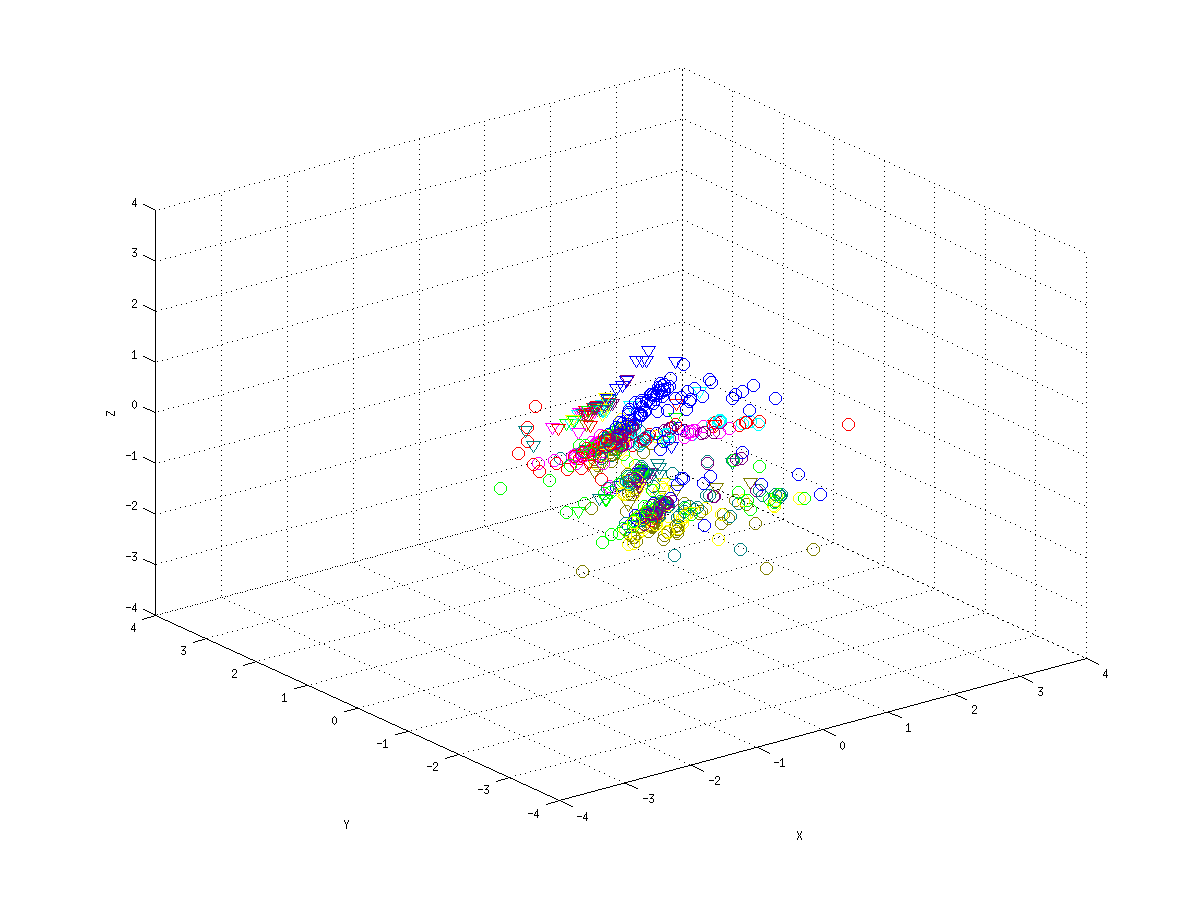
\includegraphics[width=\textwidth]{graficos/fold1_criterioParadao_reglaM_alpha0_rep1_0P.png}
                \caption{Vista en perspectiva.}
        \end{subfigure}%
        ~
        \begin{subfigure}[b]{0.49\textwidth}
                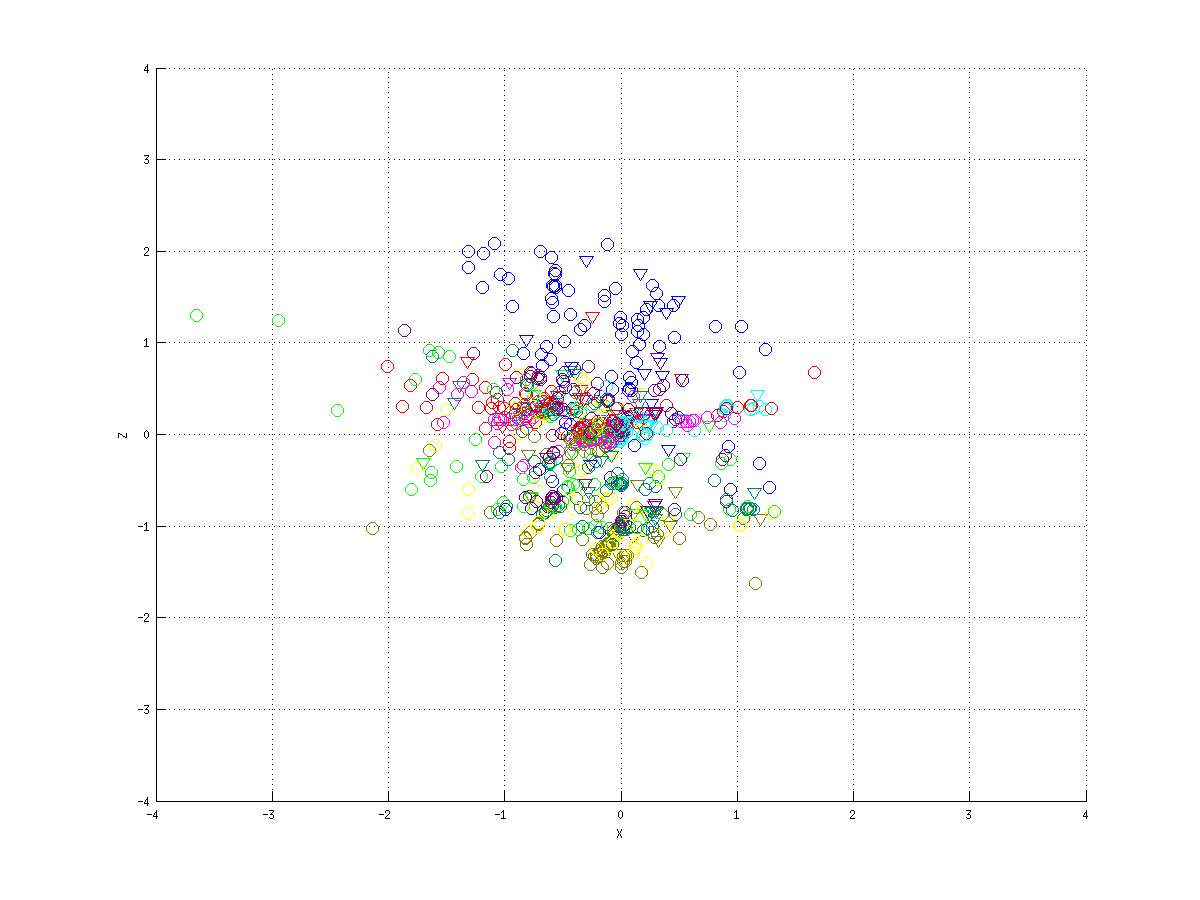
\includegraphics[width=\textwidth]{graficos/fold1_criterioParadao_reglaM_alpha0_rep1_1XZ.png}
                \caption{Plano X-Z.}
        \end{subfigure}
        
        \hspace*{-6.5cm}
        \begin{subfigure}[b]{0.49\textwidth}
                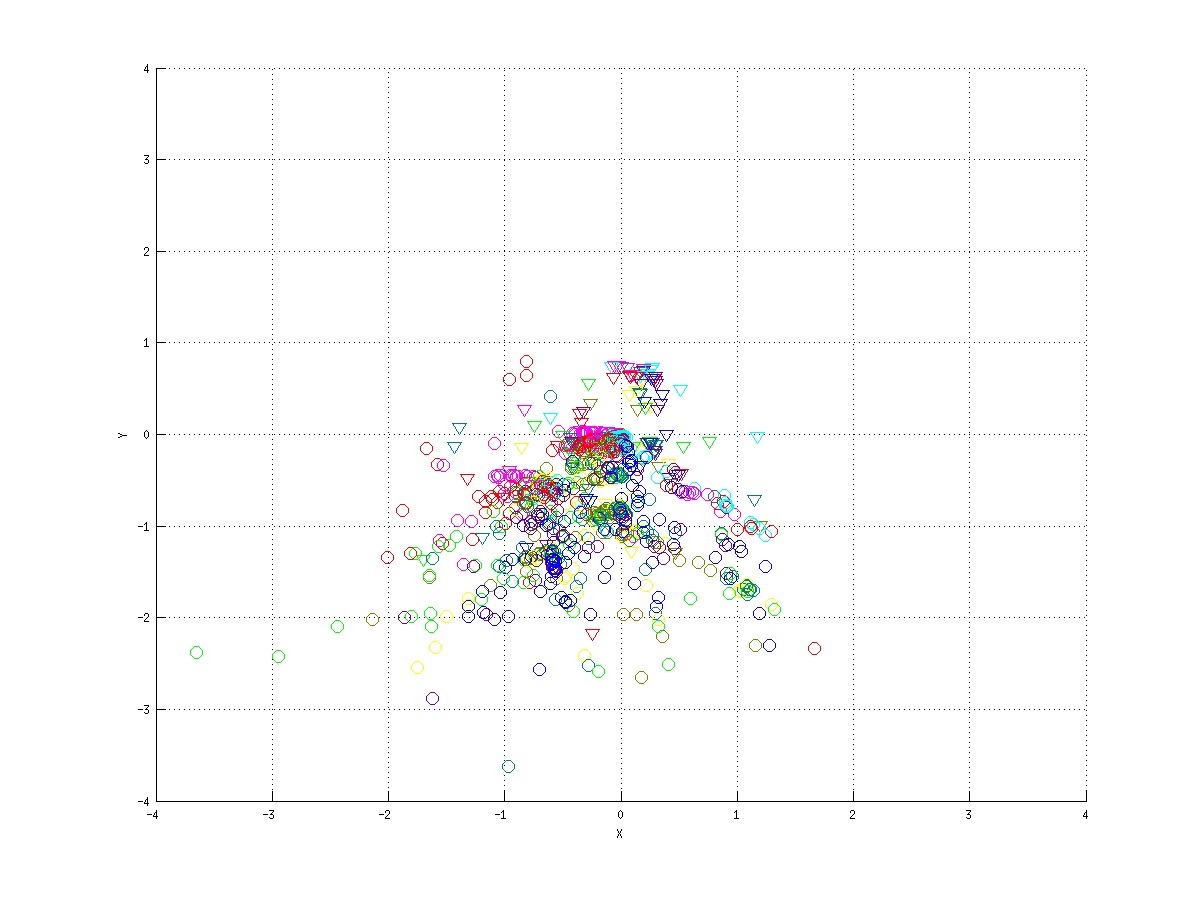
\includegraphics[width=\textwidth]{graficos/fold1_criterioParadao_reglaM_alpha0_rep1_2XY.png}
                \caption{Plano X-Y.}
        \end{subfigure}
        ~
        \begin{subfigure}[b]{0.49\textwidth}
                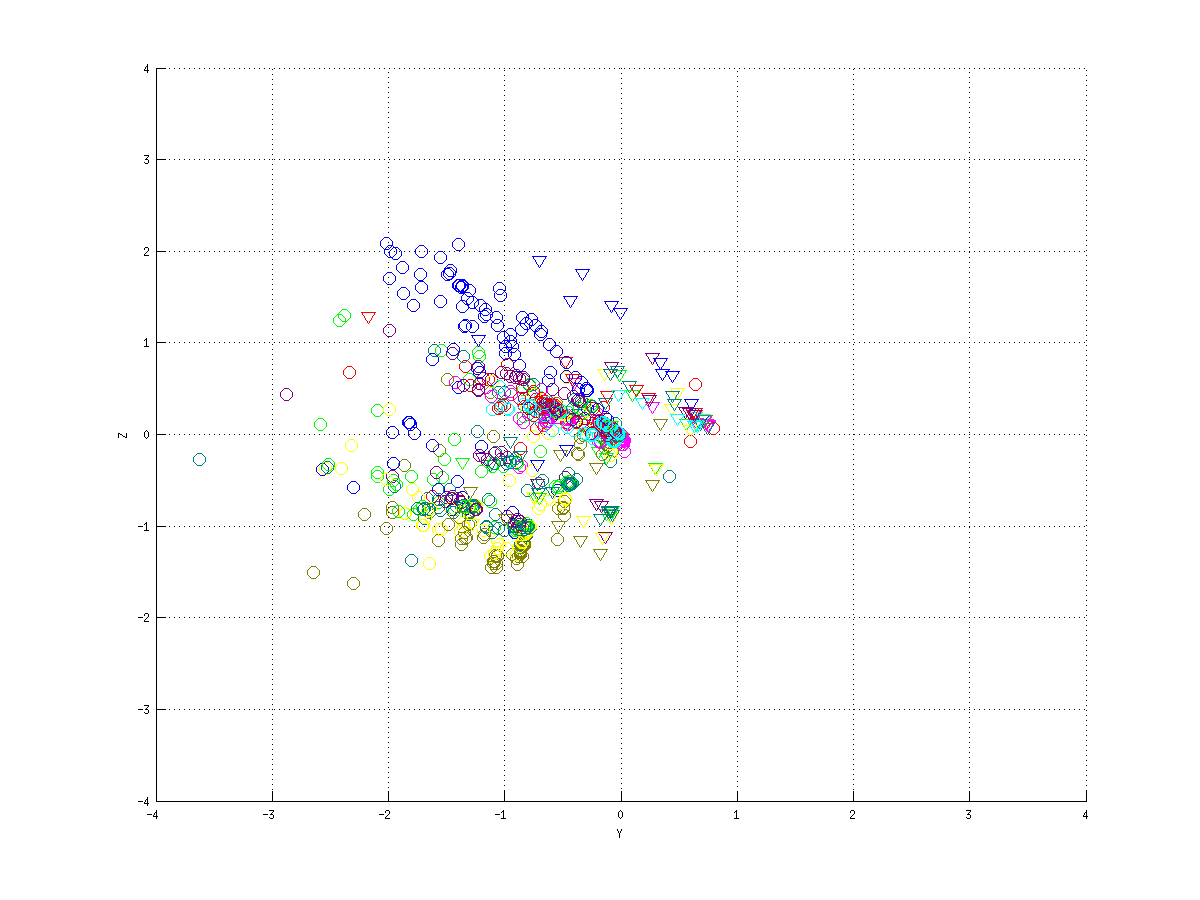
\includegraphics[width=\textwidth]{graficos/fold1_criterioParadao_reglaM_alpha0_rep1_3YZ.png}
                \caption{Plano Y-Z.}
        \end{subfigure}
	\restoregeometry
        \caption{Gráfico espacial para el Fold 1 usando ortogonalidad como criterio de parada y la regla de Oja con learning rate 0.001 en la repetición 1.}
        \label{fig:fold1_criterioParadao_reglaM_alpha0_rep1}
	\end{figure}
      
      
	\begin{figure}[H]
	\newgeometry{textwidth=21cm,textheight=21cm}
        \centering
        \hspace*{-6.5cm}
        \begin{subfigure}[b]{0.49\textwidth}
                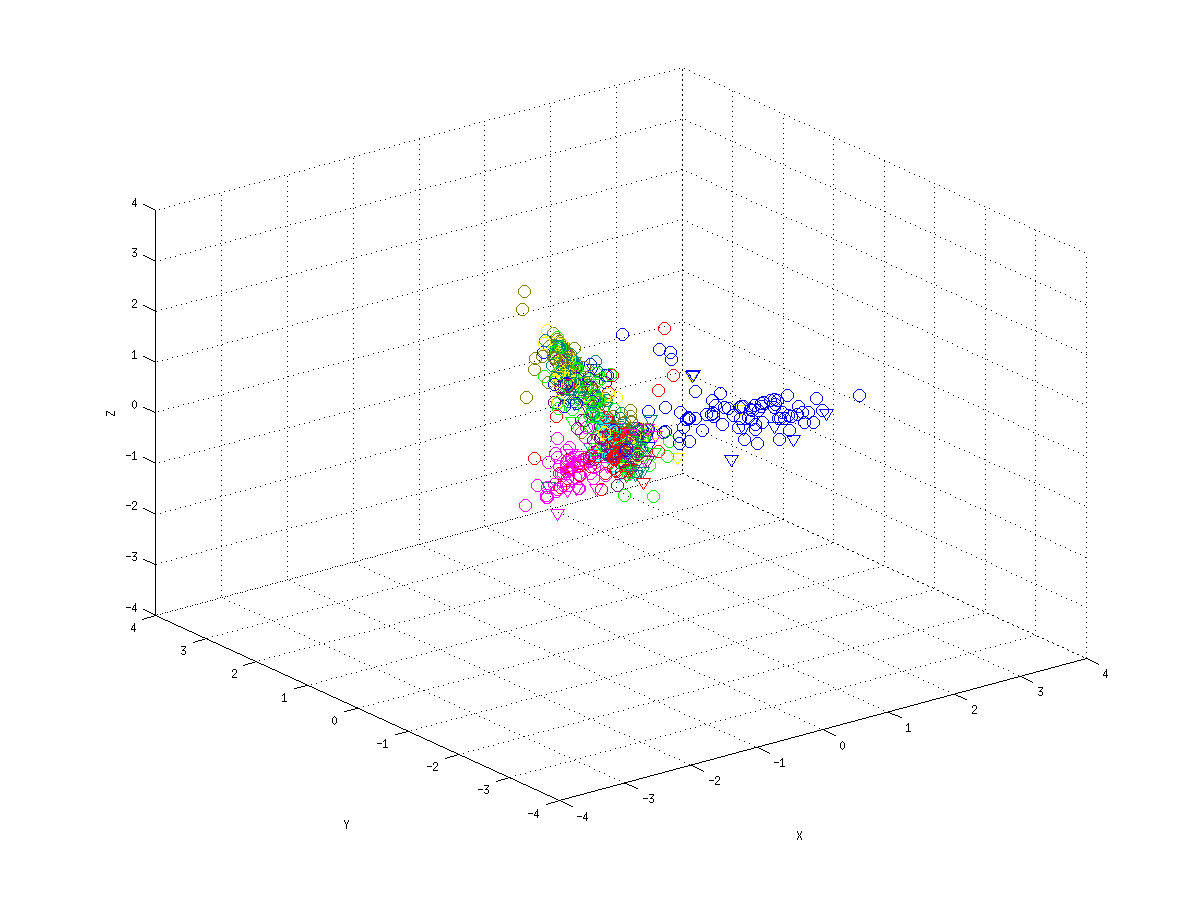
\includegraphics[width=\textwidth]{graficos/fold4_criterioParadao_reglaM_alpha0_rep3_0P.png}
                \caption{Vista en perspectiva.}
        \end{subfigure}%
        ~
        \begin{subfigure}[b]{0.49\textwidth}
                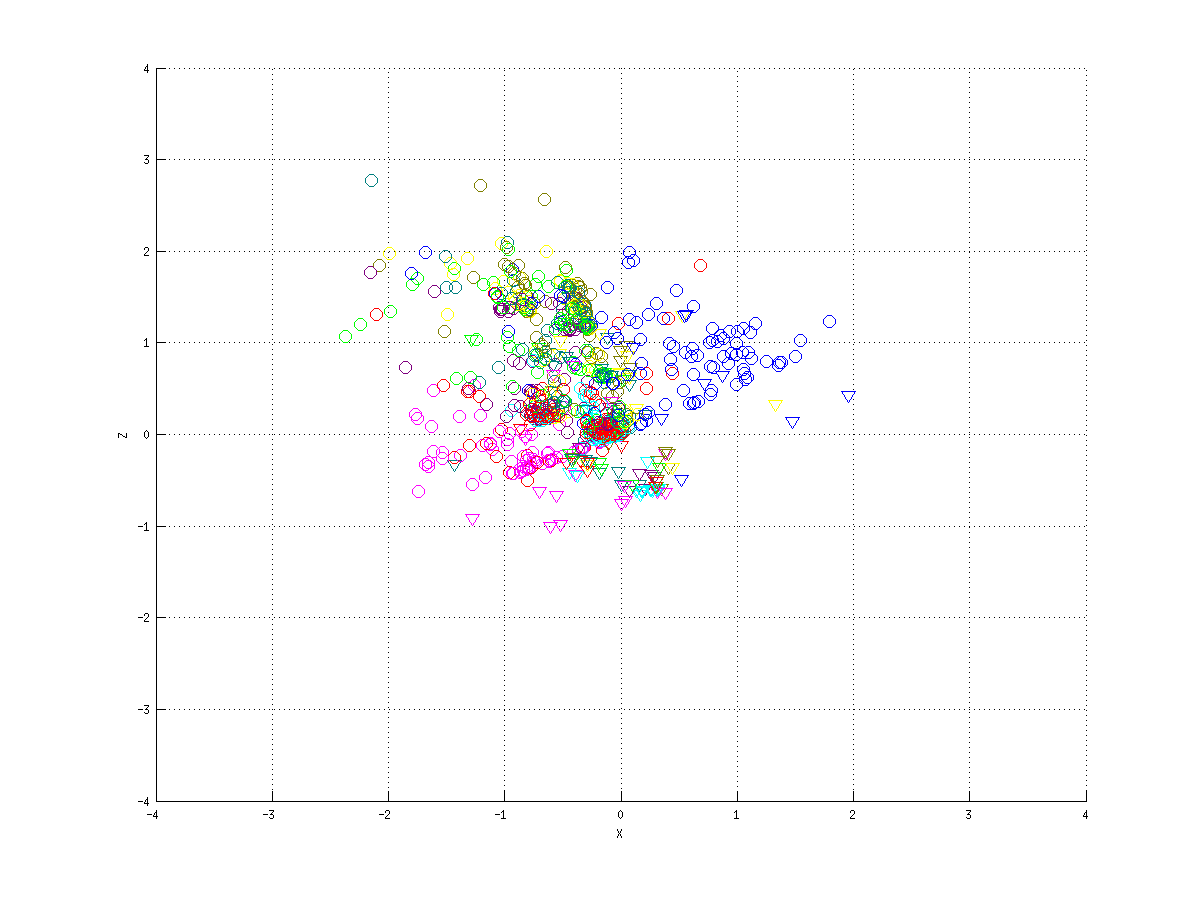
\includegraphics[width=\textwidth]{graficos/fold4_criterioParadao_reglaM_alpha0_rep3_1XZ.png}
                \caption{Plano X-Z.}
        \end{subfigure}
        
        \hspace*{-6.5cm}
        \begin{subfigure}[b]{0.49\textwidth}
                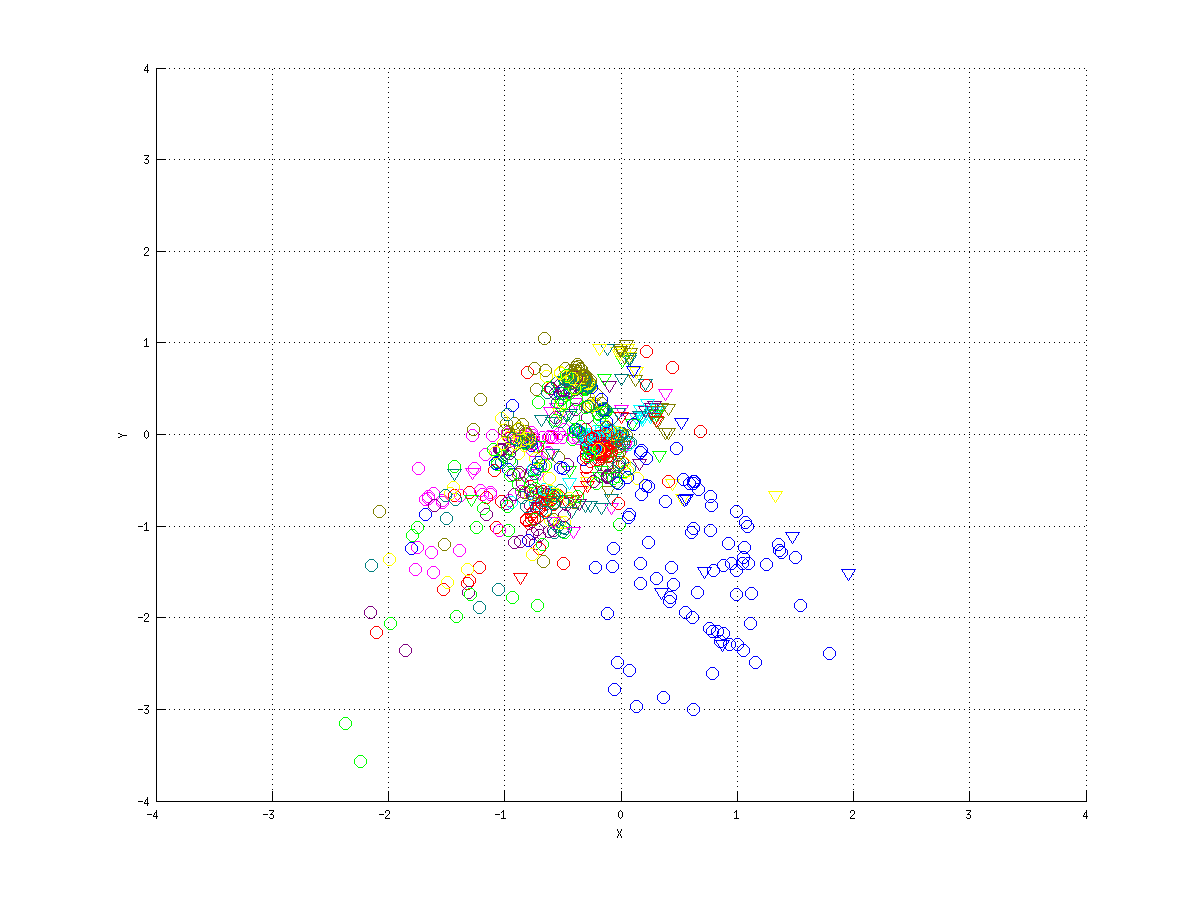
\includegraphics[width=\textwidth]{graficos/fold4_criterioParadao_reglaM_alpha0_rep3_2XY.png}
                \caption{Plano X-Y.}
        \end{subfigure}
        ~
        \begin{subfigure}[b]{0.49\textwidth}
                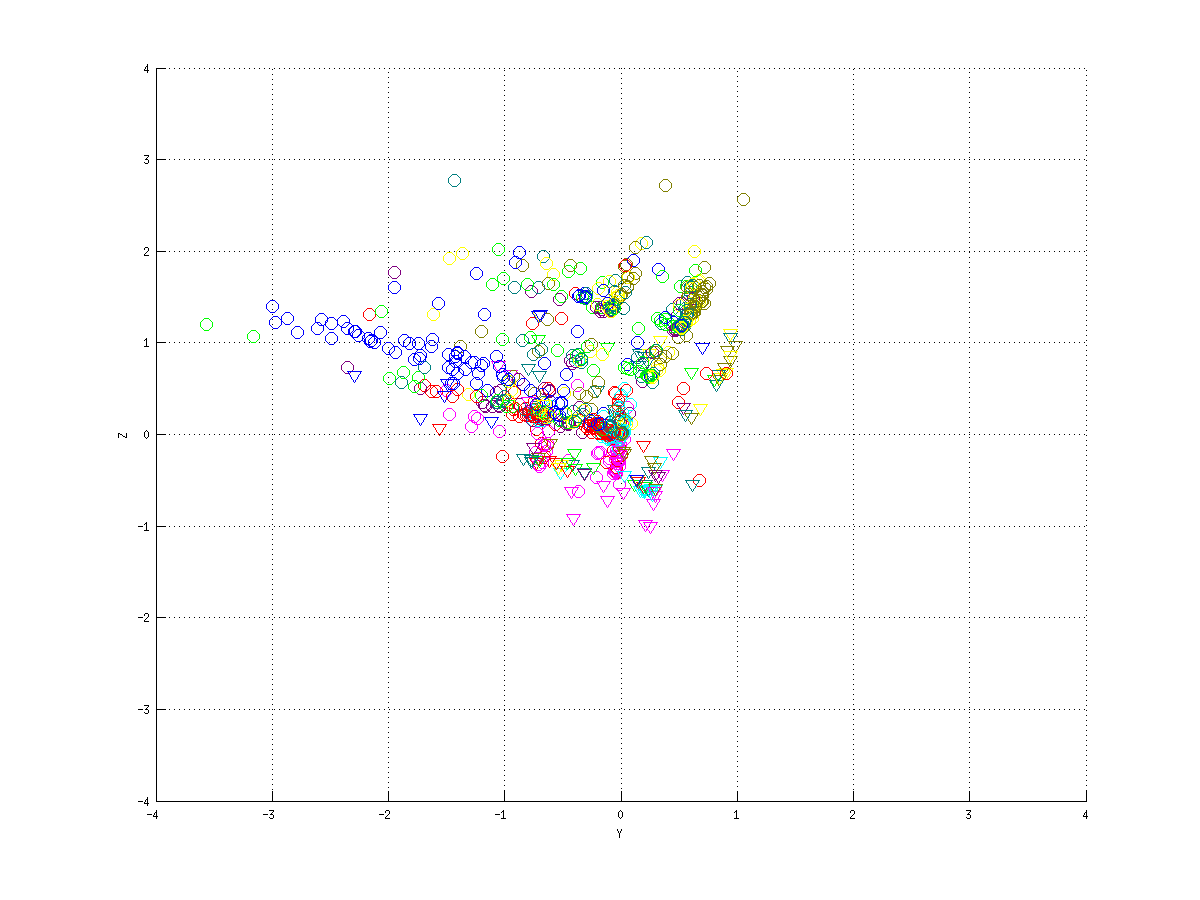
\includegraphics[width=\textwidth]{graficos/fold4_criterioParadao_reglaM_alpha0_rep3_3YZ.png}
                \caption{Plano Y-Z.}
        \end{subfigure}
	\restoregeometry
        \caption{Gráfico espacial para el Fold 4 usando ortogonalidad como criterio de parada y la regla de Oja con learning rate 0.001 en la repetición 3.}
        \label{fig:fold4_criterioParadao_reglaM_alpha0_rep3}
	\end{figure}
      
      
	\begin{figure}[H]
	\newgeometry{textwidth=21cm,textheight=21cm}
        \centering
        \hspace*{-6.5cm}
        \begin{subfigure}[b]{0.49\textwidth}
                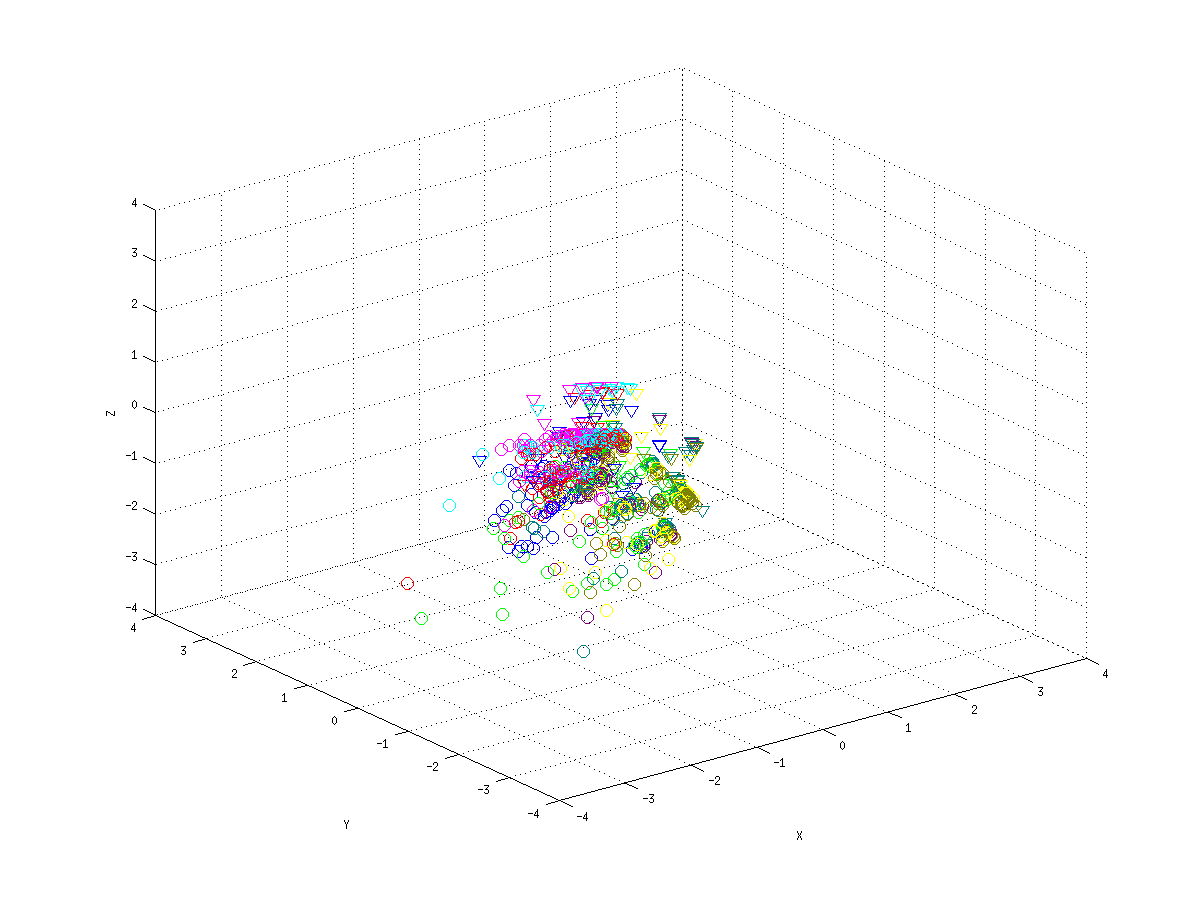
\includegraphics[width=\textwidth]{graficos/fold5_criterioParadao_reglaM_alpha0_rep2_0P.png}
                \caption{Vista en perspectiva.}
        \end{subfigure}%
        ~
        \begin{subfigure}[b]{0.49\textwidth}
                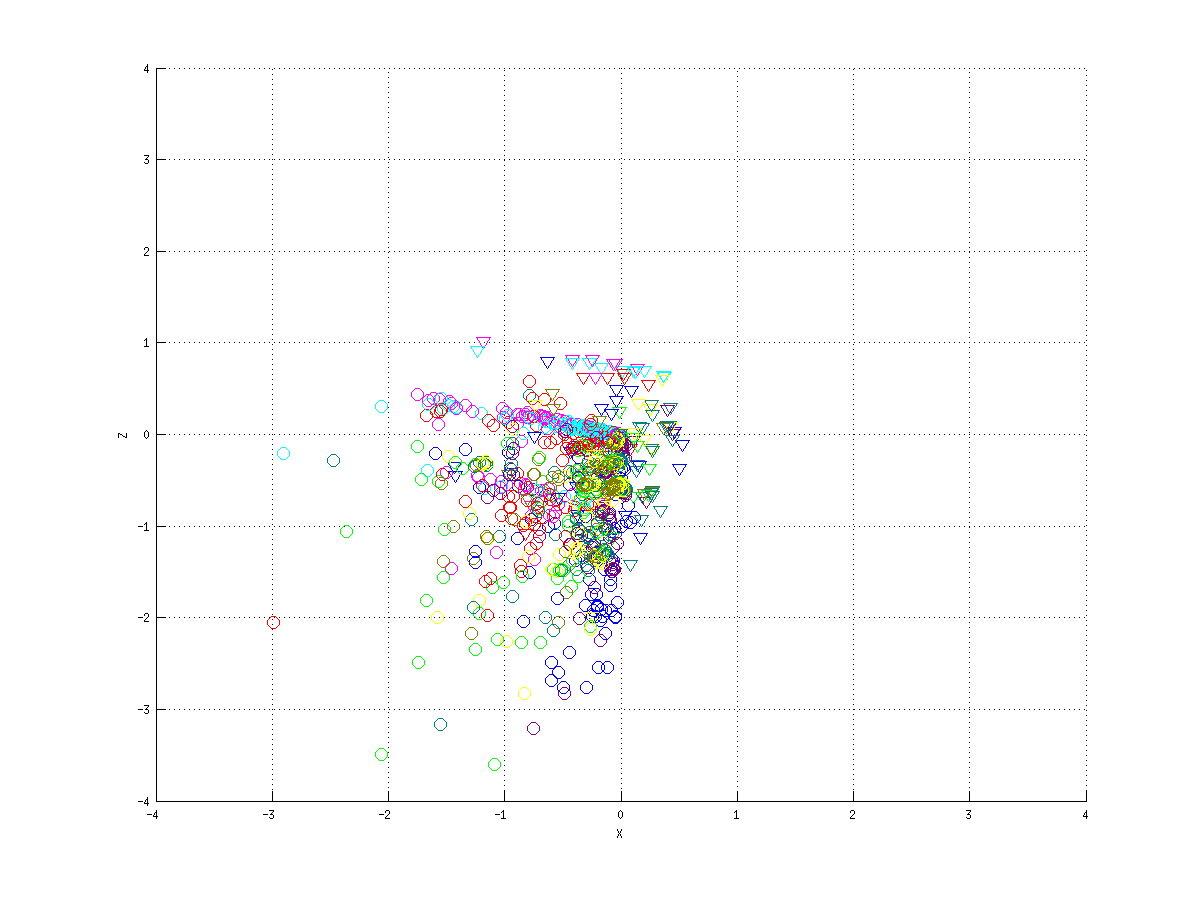
\includegraphics[width=\textwidth]{graficos/fold5_criterioParadao_reglaM_alpha0_rep2_1XZ.png}
                \caption{Plano X-Z.}
        \end{subfigure}
        
        \hspace*{-6.5cm}
        \begin{subfigure}[b]{0.49\textwidth}
                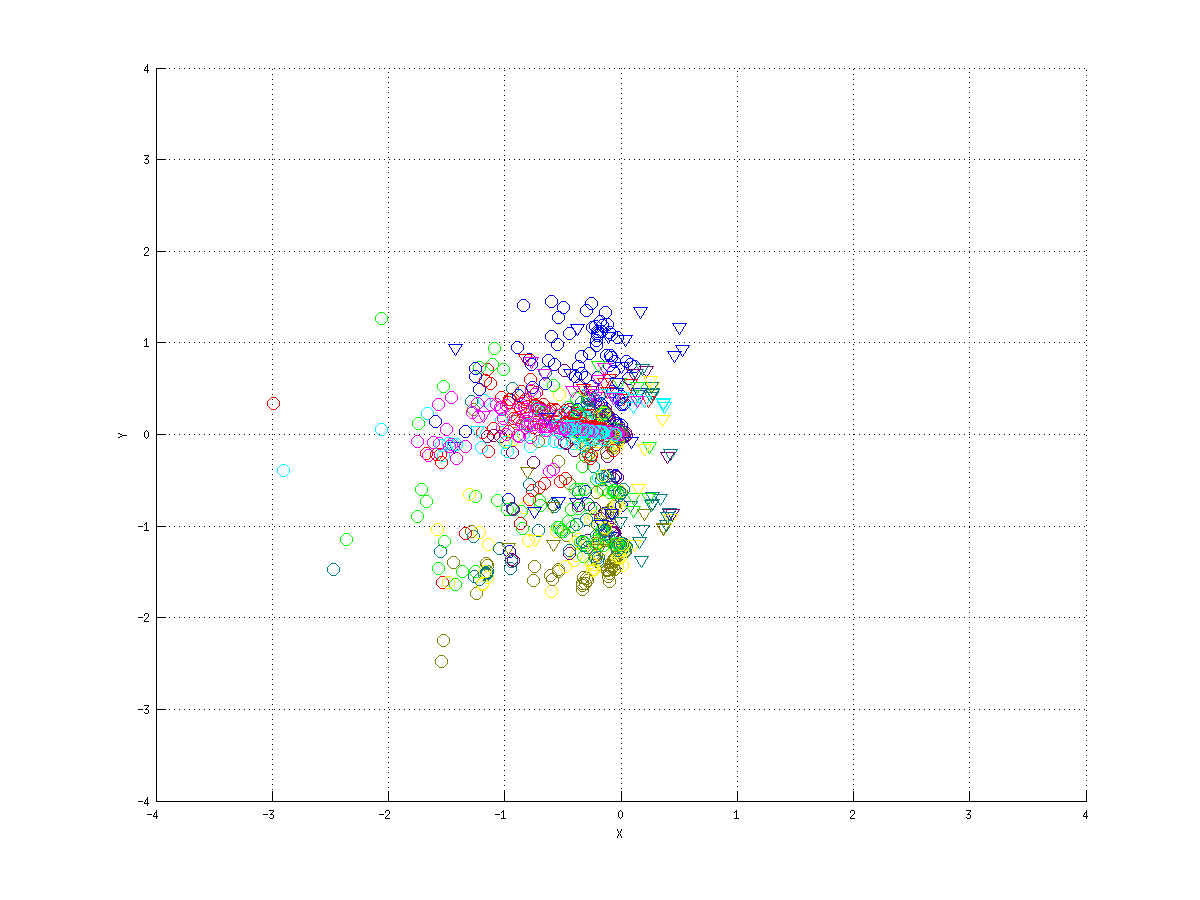
\includegraphics[width=\textwidth]{graficos/fold5_criterioParadao_reglaM_alpha0_rep2_2XY.png}
                \caption{Plano X-Y.}
        \end{subfigure}
        ~
        \begin{subfigure}[b]{0.49\textwidth}
                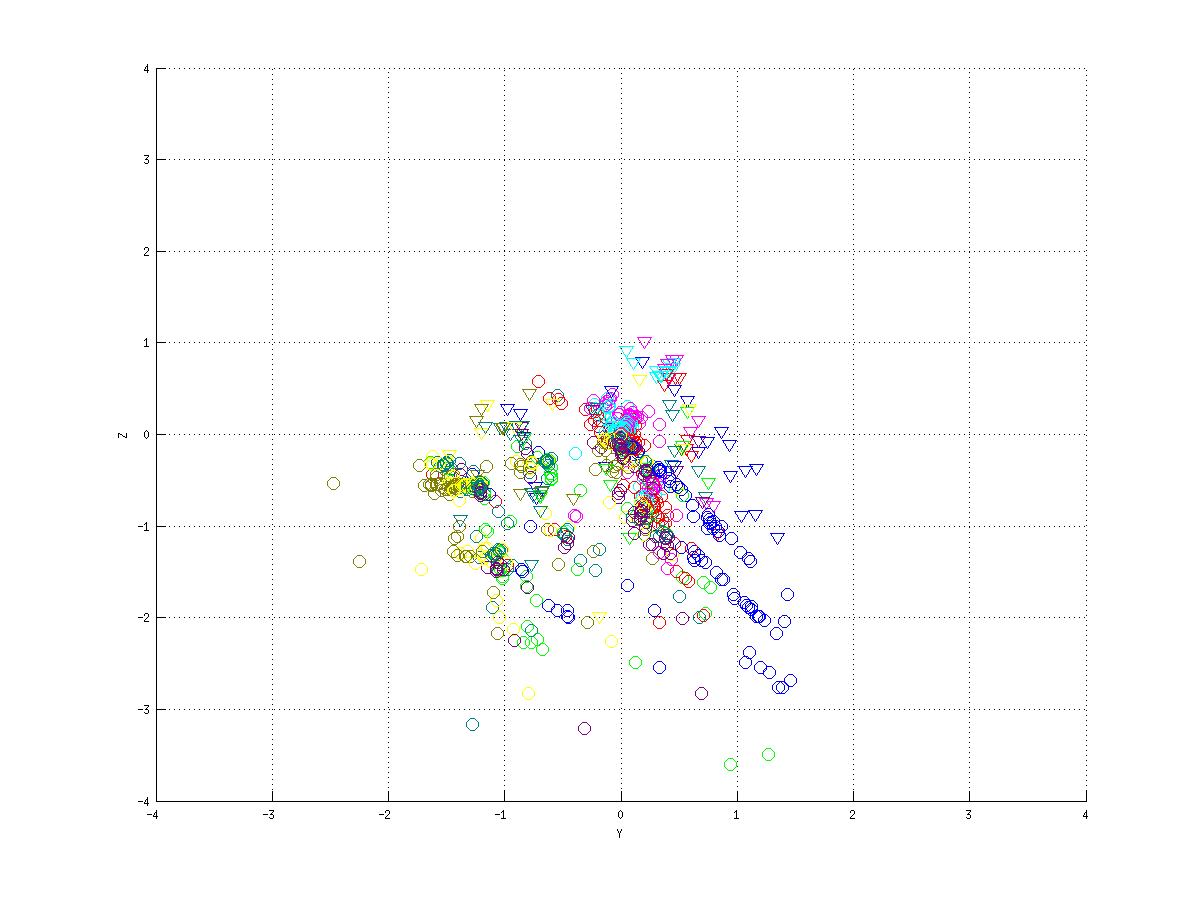
\includegraphics[width=\textwidth]{graficos/fold5_criterioParadao_reglaM_alpha0_rep2_3YZ.png}
                \caption{Plano Y-Z.}
                \label{fig:fold5_criterioParadao_reglaM_alpha0_rep2_3YZ}
        \end{subfigure}
	\restoregeometry
        \caption{Gráfico espacial para el Fold 5 usando ortogonalidad como criterio de parada y la regla de Oja con learning rate 0.001 en la repetición 2.}
        \label{fig:fold5_criterioParadao_reglaM_alpha0_rep2}
	\end{figure}
      
      
	\begin{figure}[H]
	\newgeometry{textwidth=21cm,textheight=21cm}
        \centering
        \hspace*{-6.5cm}
        \begin{subfigure}[b]{0.49\textwidth}
                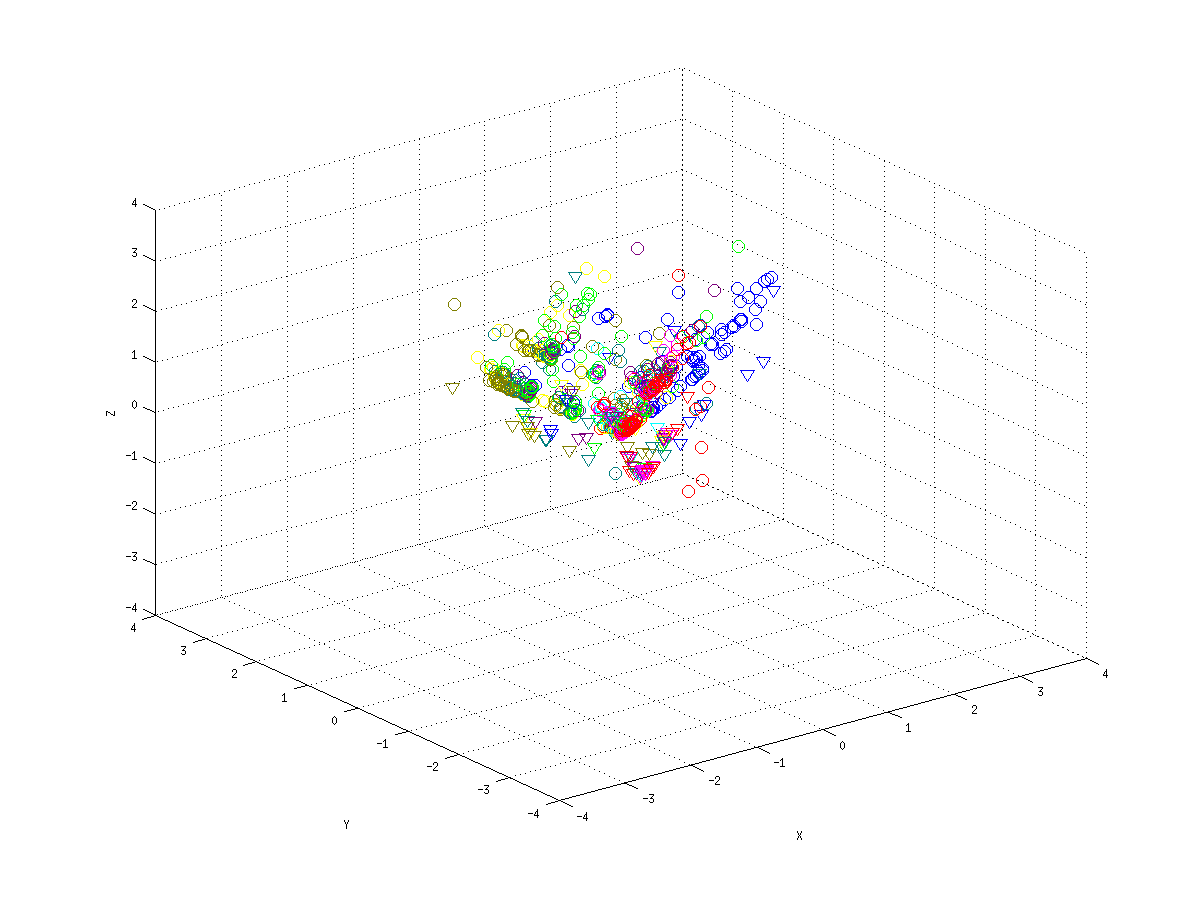
\includegraphics[width=\textwidth]{graficos/fold7_criterioParadao_reglaM_alpha0_rep4_0P.png}
                \caption{Vista en perspectiva.}
        \end{subfigure}%
        ~
        \begin{subfigure}[b]{0.49\textwidth}
                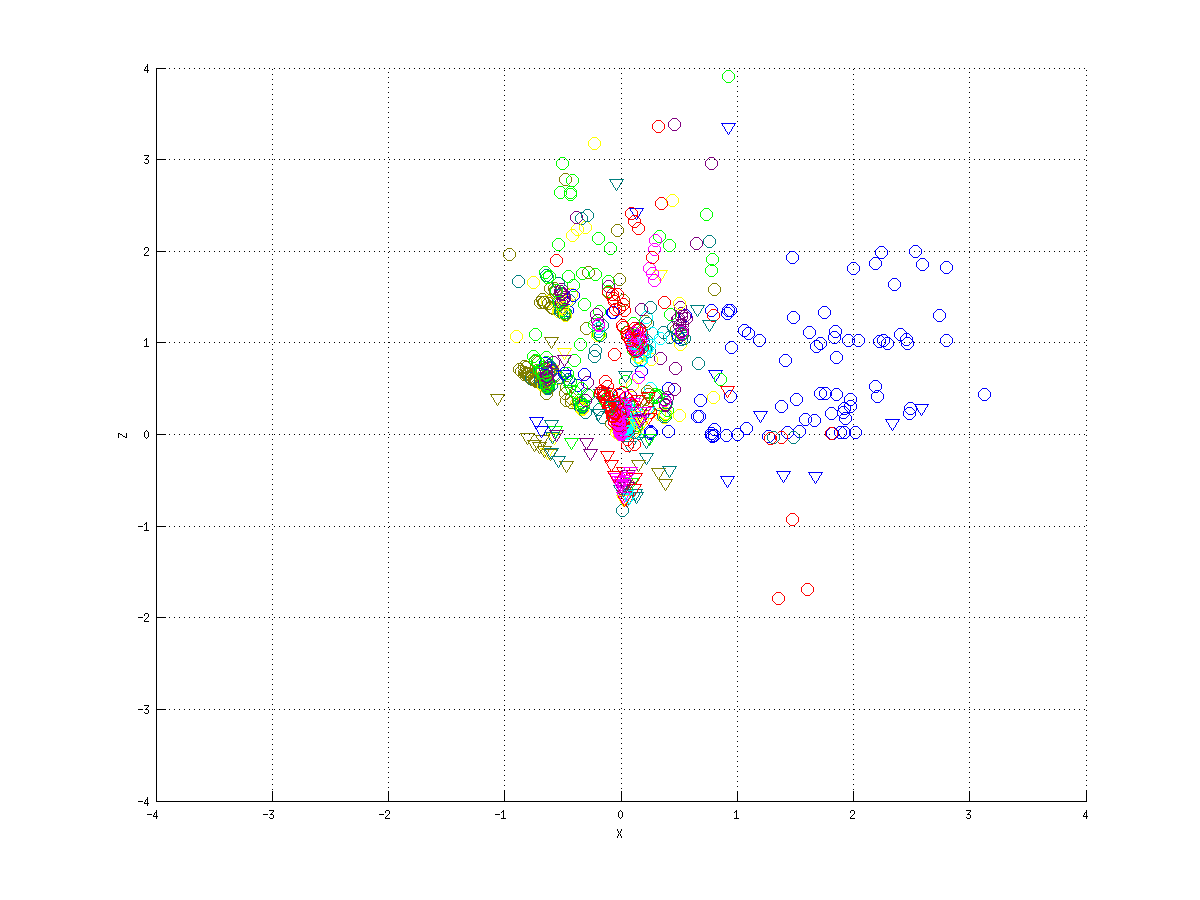
\includegraphics[width=\textwidth]{graficos/fold7_criterioParadao_reglaM_alpha0_rep4_1XZ.png}
                \caption{Plano X-Z.}
        \end{subfigure}
        
        \hspace*{-6.5cm}
        \begin{subfigure}[b]{0.49\textwidth}
                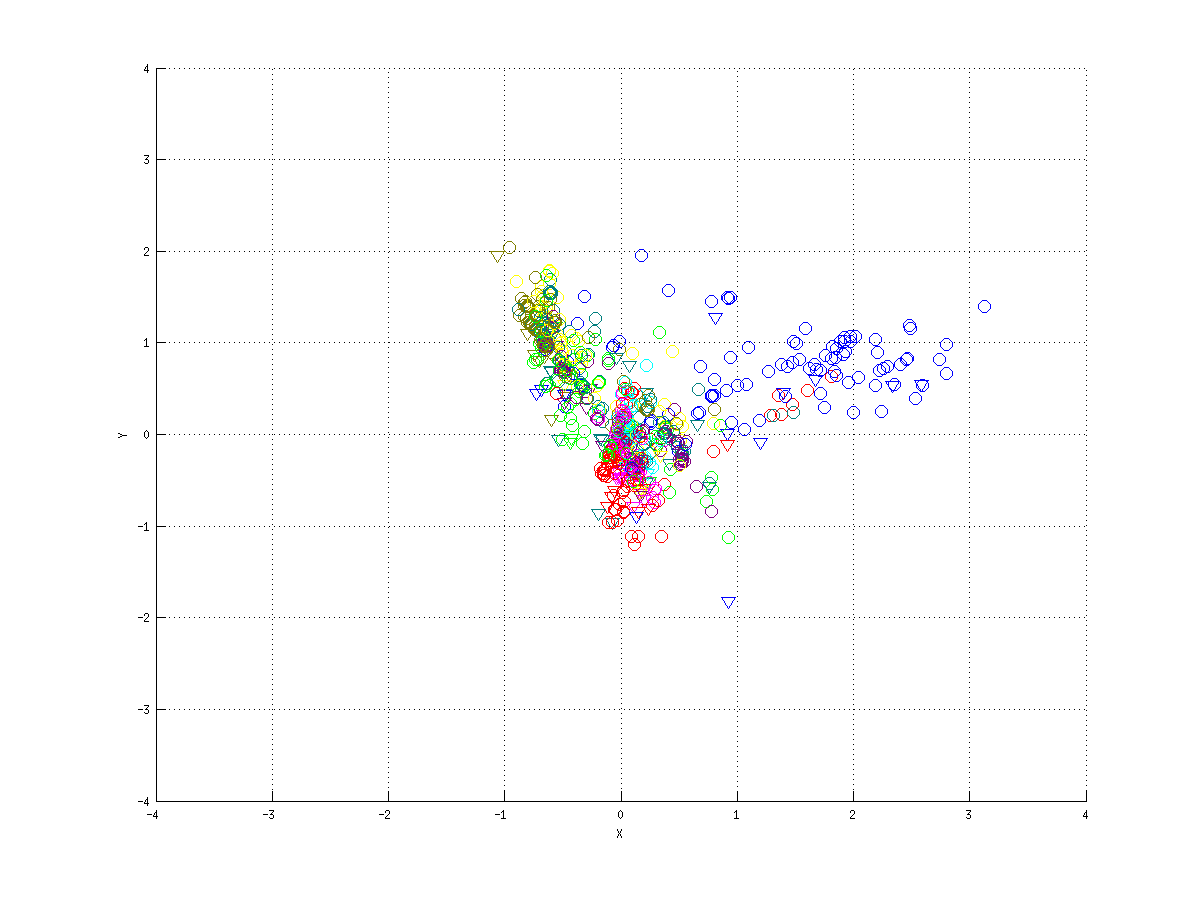
\includegraphics[width=\textwidth]{graficos/fold7_criterioParadao_reglaM_alpha0_rep4_2XY.png}
                \caption{Plano X-Y.}
        \end{subfigure}
        ~
        \begin{subfigure}[b]{0.49\textwidth}
                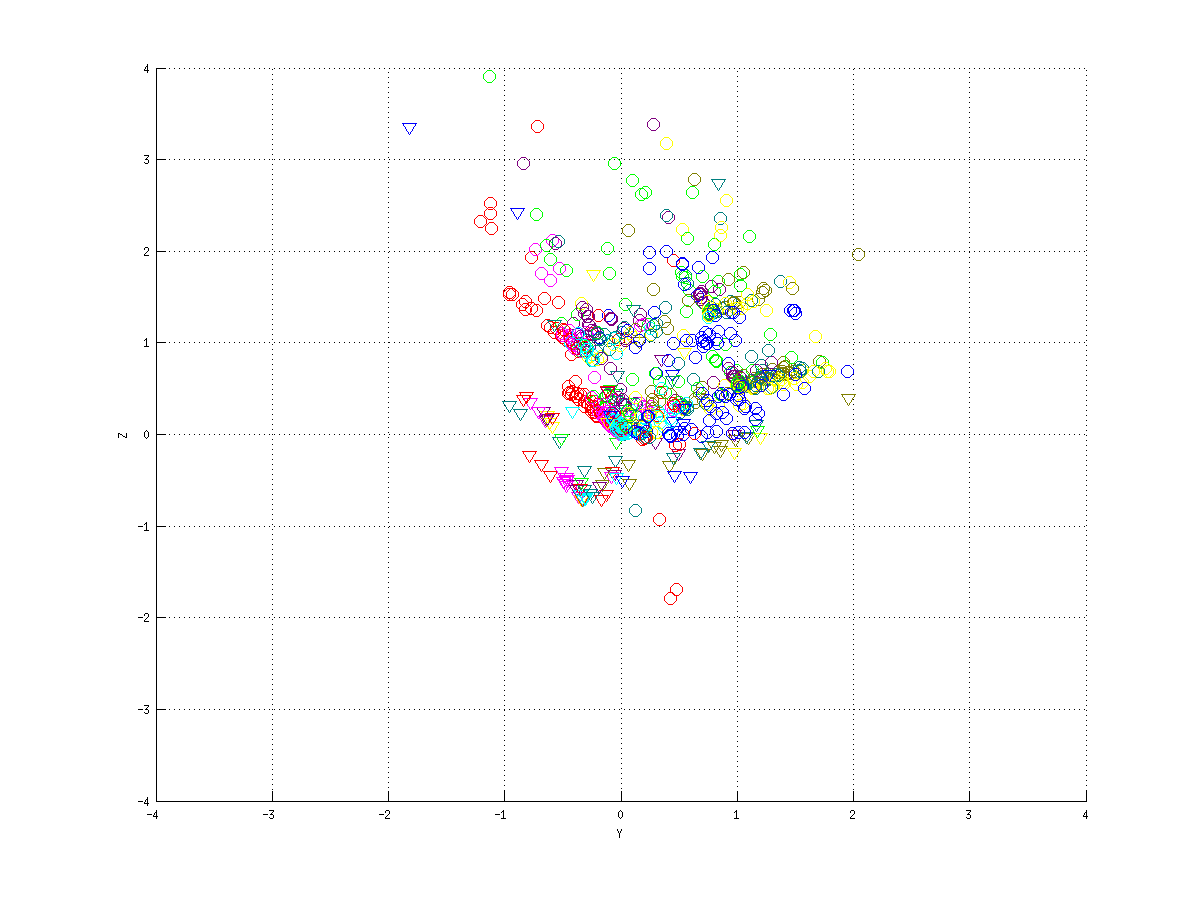
\includegraphics[width=\textwidth]{graficos/fold7_criterioParadao_reglaM_alpha0_rep4_3YZ.png}
                \caption{Plano Y-Z.}
        \end{subfigure}
	\restoregeometry
        \caption{Gráfico espacial para el Fold 7 usando ortogonalidad como criterio de parada y la regla de Oja con learning rate 0.001 en la repetición 4.}
        \label{fig:fold7_criterioParadao_reglaM_alpha0_rep4}
	\end{figure}
      
      
      
      
      \myparagraph{Particularidades con regla de Sanger y criterio de ortogonalidad}
      
	De manera similar al caso anterior, decidimos mostrar algunos de los resultados que de alguna manera representan a la mayoría. Vale aclarar que no se observaron diferencias significativas entre los casos en los cuales se convergió por criterio de ortogonalidad y por máximo de épocas.
	
	Por un lado, en la Figura \ref{fig:fold2_criterioParadao_reglas_alpha0_rep4} se ve cómo las distintas clases no se encuentran espacialmente muy dispersas. Apenas la clase azul está un poco alejada de las demás. El resto de las clases aparecen en pequeños cúmulos como la roja, violeta, magenta, verde, amarilla y marrón. Las restantes están un poco más dispersas.
	
	Por otro lado, en la Figura \ref{fig:fold1_criterioParadao_reglas_alpha0_rep4} se ve a simple vista cómo la clase azul ocupa un lugar más alejado del resto de las clases mientras que las otras clases aparecen más juntas entre sí. De todos modos es posible ver algunos cúmulos como el ocupado por las clases verde, amarilla y marrón. La clase roja, a diferencia del caso analizado anteriormente, aparece más dispersa.
      
	~
	
	De manera análoga a lo observado al usar la regla de Oja, es posible ver que salvo casos particulares, tanto las instancias de entrenamiento como las de validación ocupan los mismos lugares en el espacio por lo que es posible que al realizar una clasificación posterior, el uso de las tres componentes principales permitan obtener buenos resultados. Al igual que antes, desde lo visual no se pueden diferenciar zonas claras para cada color aunque sí algunos cúmulos ocupados específicamente por ciertas clases.
      
	\begin{figure}[H]
	\newgeometry{textwidth=21cm,textheight=21cm}
        \centering
        \hspace*{-6.5cm}
        \begin{subfigure}[b]{0.49\textwidth}
                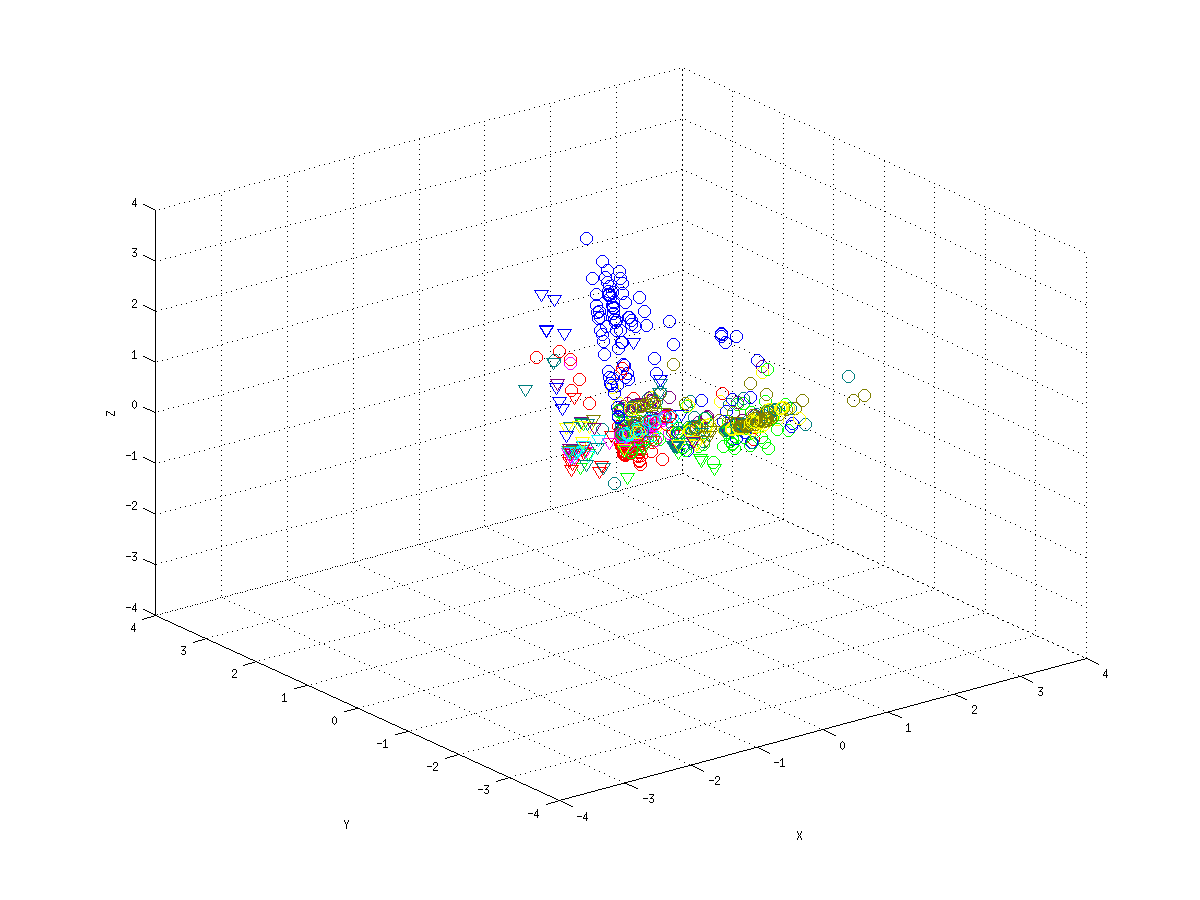
\includegraphics[width=\textwidth]{graficos/fold1_criterioParadao_reglas_alpha0_rep4_0P.png}
                \caption{Vista en perspectiva.}
        \end{subfigure}%
        ~
        \begin{subfigure}[b]{0.49\textwidth}
                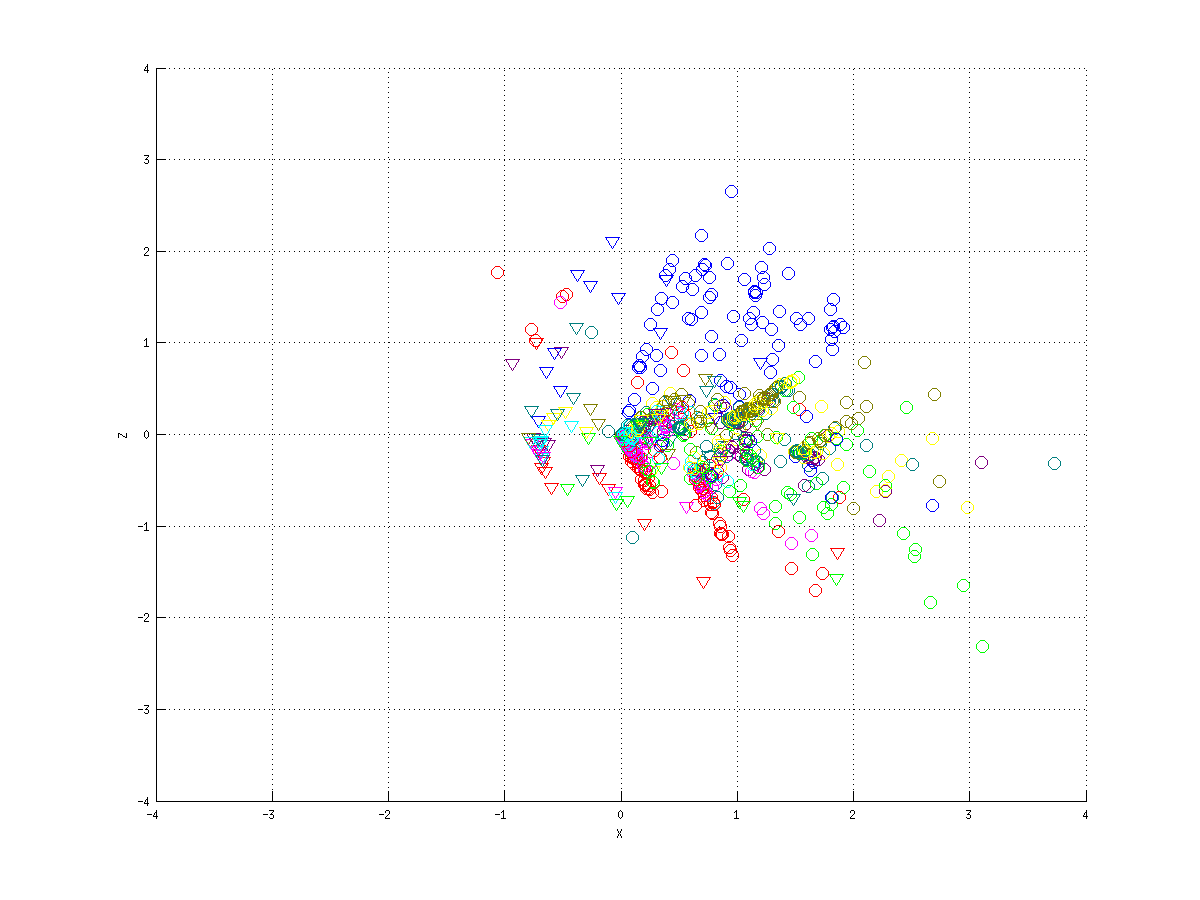
\includegraphics[width=\textwidth]{graficos/fold1_criterioParadao_reglas_alpha0_rep4_1XZ.png}
                \caption{Plano X-Z.}
        \end{subfigure}
        
        \hspace*{-6.5cm}
        \begin{subfigure}[b]{0.49\textwidth}
                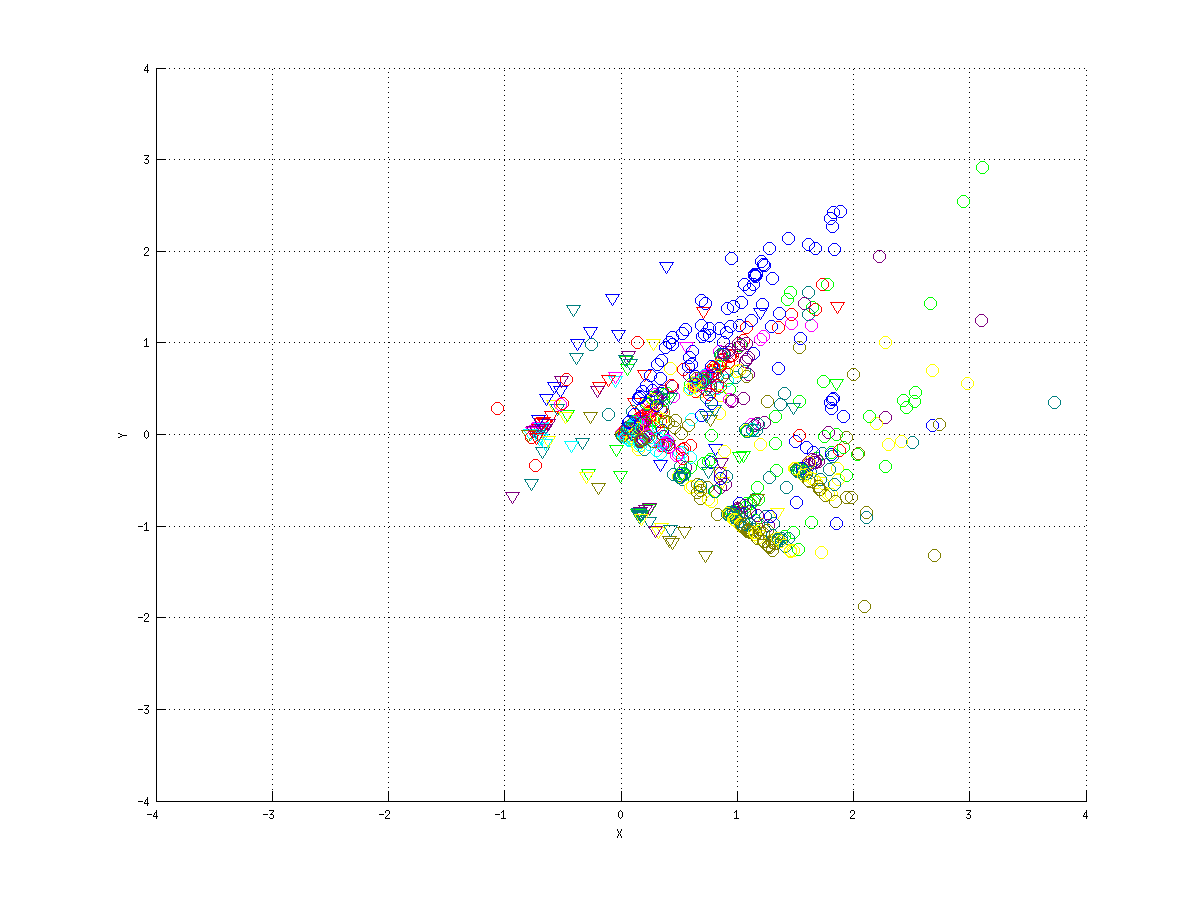
\includegraphics[width=\textwidth]{graficos/fold1_criterioParadao_reglas_alpha0_rep4_2XY.png}
                \caption{Plano X-Y.}
        \end{subfigure}
        ~
        \begin{subfigure}[b]{0.49\textwidth}
                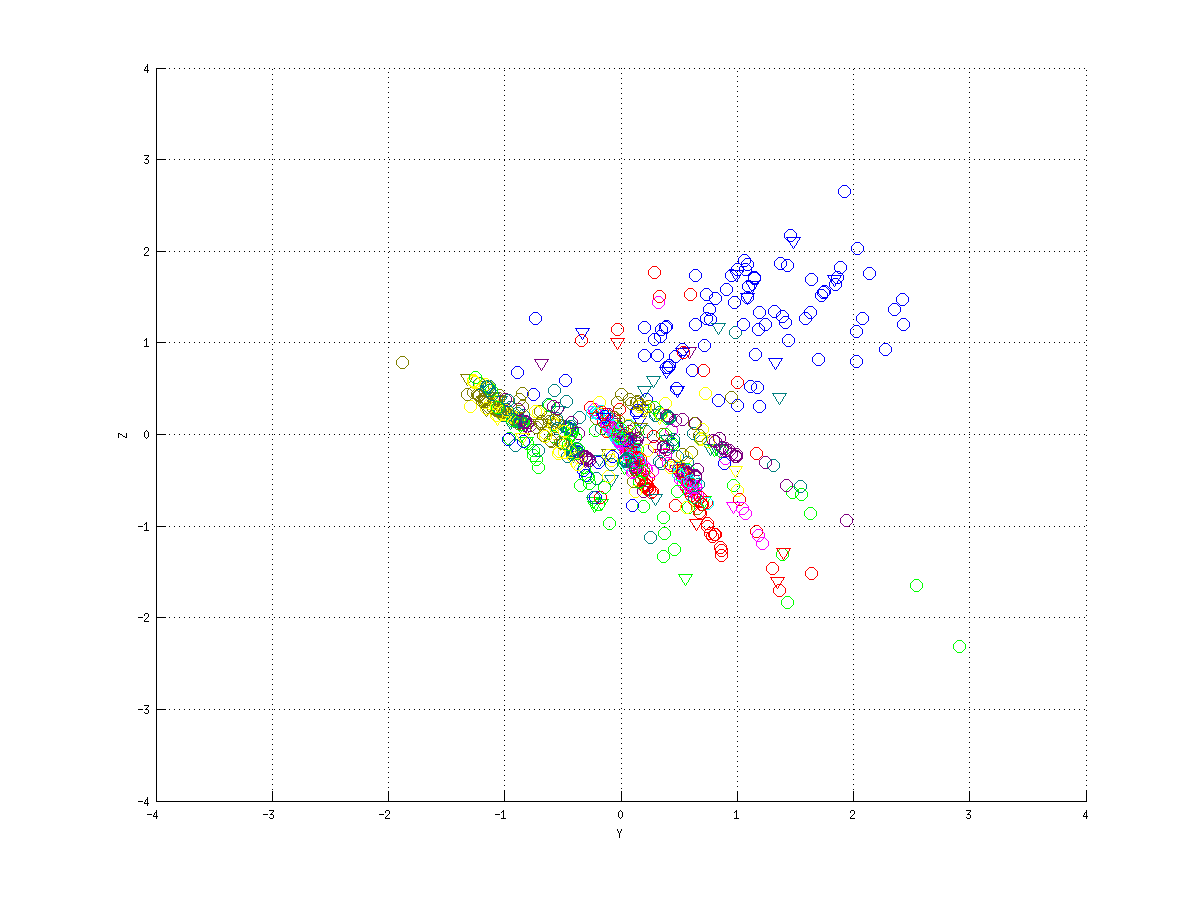
\includegraphics[width=\textwidth]{graficos/fold1_criterioParadao_reglas_alpha0_rep4_3YZ.png}
                \caption{Plano Y-Z.}
        \end{subfigure}
	\restoregeometry
        \caption{Gráfico espacial para el Fold 1 usando ortogonalidad como criterio de parada y la regla de Sanger con learning rate 0.001 en la repetición 4.}
        \label{fig:fold1_criterioParadao_reglas_alpha0_rep4}
	\end{figure}
      
	
	\begin{figure}[H]
	\newgeometry{textwidth=21cm,textheight=21cm}
        \centering
        \hspace*{-6.5cm}
        \begin{subfigure}[b]{0.49\textwidth}
                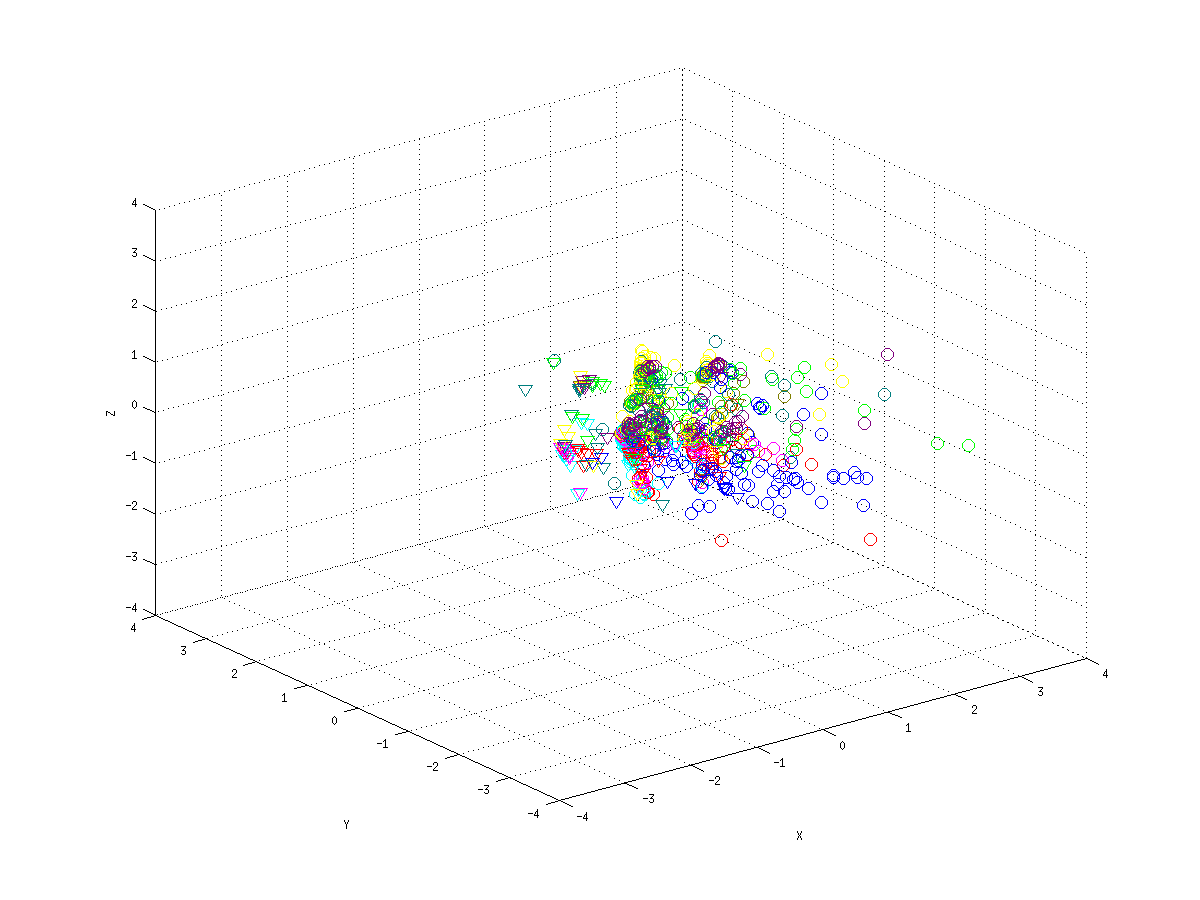
\includegraphics[width=\textwidth]{graficos/fold2_criterioParadao_reglas_alpha0_rep4_0P.png}
                \caption{Vista en perspectiva.}
        \end{subfigure}%
        ~
        \begin{subfigure}[b]{0.49\textwidth}
                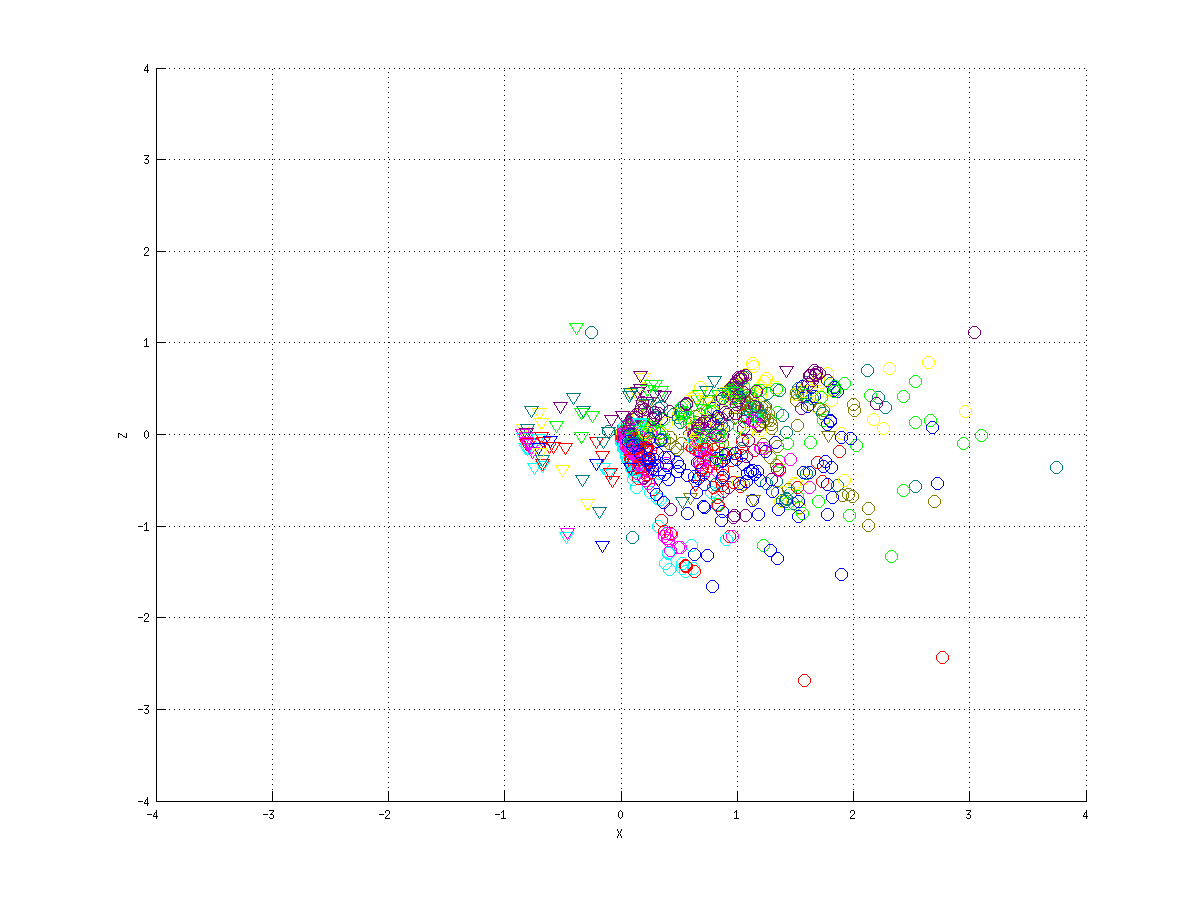
\includegraphics[width=\textwidth]{graficos/fold2_criterioParadao_reglas_alpha0_rep4_1XZ.png}
                \caption{Plano X-Z.}
        \end{subfigure}
        
        \hspace*{-6.5cm}
        \begin{subfigure}[b]{0.49\textwidth}
                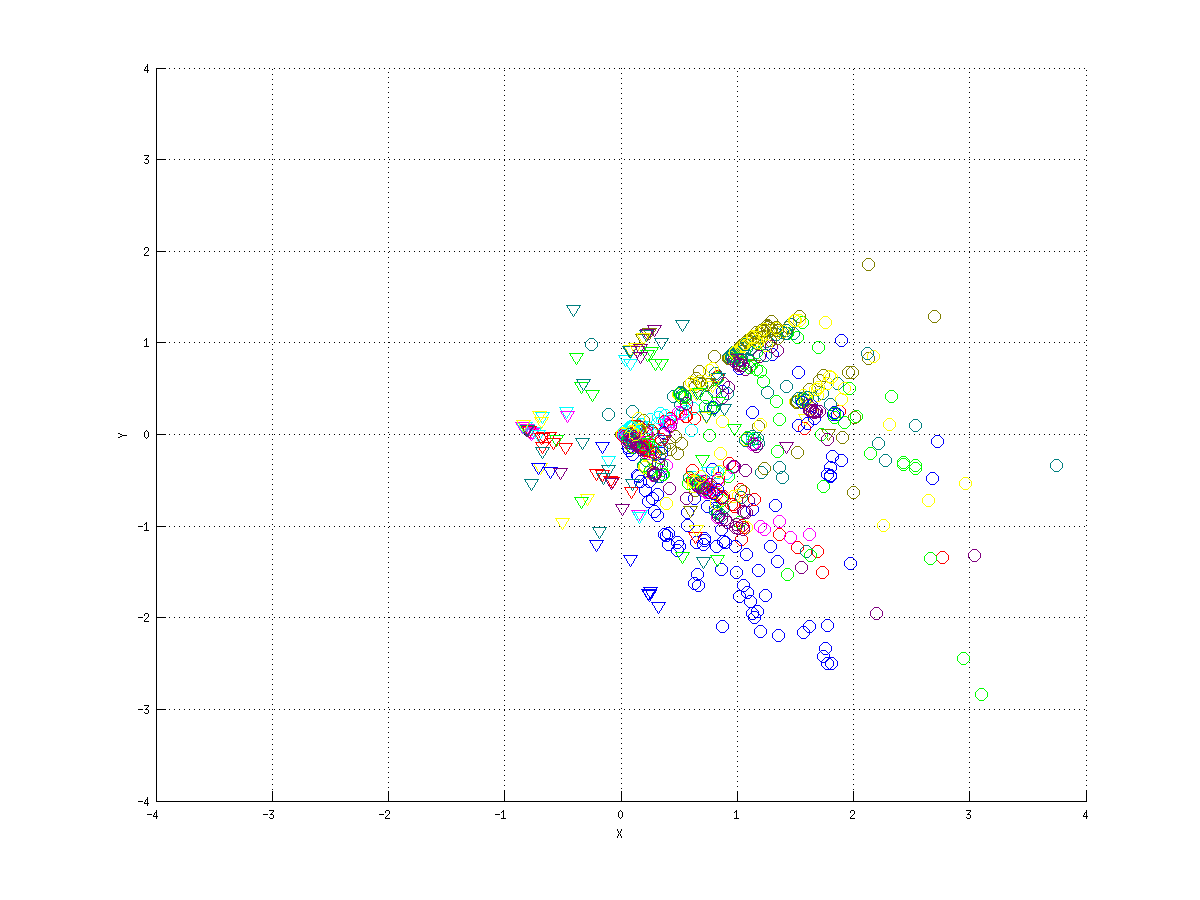
\includegraphics[width=\textwidth]{graficos/fold2_criterioParadao_reglas_alpha0_rep4_2XY.png}
                \caption{Plano X-Y.}
        \end{subfigure}
        ~
        \begin{subfigure}[b]{0.49\textwidth}
                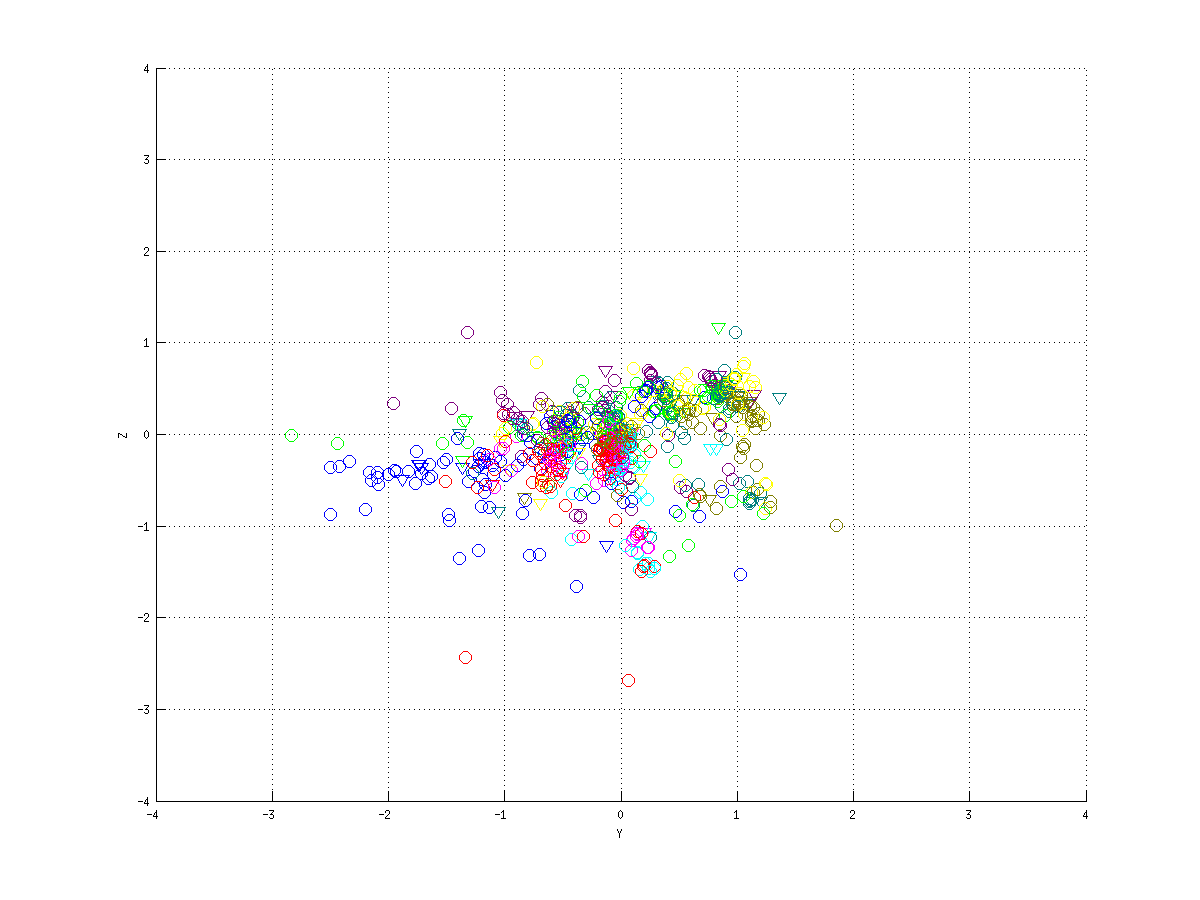
\includegraphics[width=\textwidth]{graficos/fold2_criterioParadao_reglas_alpha0_rep4_3YZ.png}
                \caption{Plano Y-Z.}
        \end{subfigure}
	\restoregeometry
        \caption{Gráfico espacial para el Fold 2 usando ortogonalidad como criterio de parada y la regla de Sanger con learning rate 0.001 en la repetición 4.}
        \label{fig:fold2_criterioParadao_reglas_alpha0_rep4}
	\end{figure}
      
      
      
      
      
      
      
      
      \myparagraph{Particularidades con regla de Oja y criterio de $\Delta W$}
      
	A continuación presentamos resultados correspondientes al uso de la regla de Oja con el criterio de la matriz de delta de pesos. Recordando de las Tablas \ref{tab:pesos_oja500} y \ref{tab:pesos_oja250} que en casi todos los casos se produjo el corte por alcanzar un valor muy bajo en la matriz de pesos.
	
	En la Figura \ref{fig:fold1_criterioParadap_reglaM_alpha0_rep2} se observa el patrón más veces repetido entre los experimentos. En dicho gráfico se ve que las instancias de la clase azul ocupan una porción alejada del resto de las instancias mientras que el resto se ubican mucho más juntas. En ellas hay varios cúmulos donde se encuentran las clases roja y celeste juntas por un lado rodeadas de la magenta y un poco más alejadas las verde, amarilla y marrón. Las clases violeta y azul oscuro aparecen junto a los cúmulos pero más esparcidas en el espacio.
	
	La Figura \ref{fig:fold6_criterioParadap_reglaM_alpha0_rep3} presenta un caso particular en el cual varias instancias se ubican formando casi una línea recta sobre el eje X, correspondiente a la componente principal. Al igual que en los casos anteriores la clase azul ocupa un lugar más alejado que el resto de las clases. Principalmente las clases roja y magenta tienen a sus instancias ubicadas casi en línea recta indicando que el mayor peso para esas instancias es respecto de la componente principal. Observando el conjunto de entrenamiento y los resultados no se ve ninguna característica a simple vista de modo que intuímos que el resultado tiene que ver con el orden de entrenamiento y los pesos iniciales de la matriz de pesos.
	
	De manera similar al caso anterior, las clases amarilla, verde y marrón se ubican en los mismos cúmulos y por otro lado las instancias de la clase celeste aparecen bien concentradas. El resto de las clases aparecen distribuídas sin seguir ningún patrón fácilmente identificable en los gráficos.
	
	~
	
	Considerando las instancias de validación, en los gráficos no se ven muchas de ellas alejadas de las de entrenamiento ubicadas en lugares demasiado distintos. De manera visual, esto indica que la separación en tres dimensiones de esta técnica permite diferenciar bastante bien las clases. Es claro que no es posible asegurar este comportamiento de esta manera por lo que sería necesario aplicar posteriormente alguna técnica de clasificación para analizar cuantitativamente los resultados. La Principal ventaja de este conjunto de parámetros es que en una cantidad de épocas mucho menor se alcanzaron resultados muy similares a las combinaciones discutidas anteriormente.
      
	\begin{figure}[H]
	\newgeometry{textwidth=21cm,textheight=21cm}
        \centering
        \hspace*{-6.5cm}
        \begin{subfigure}[b]{0.49\textwidth}
                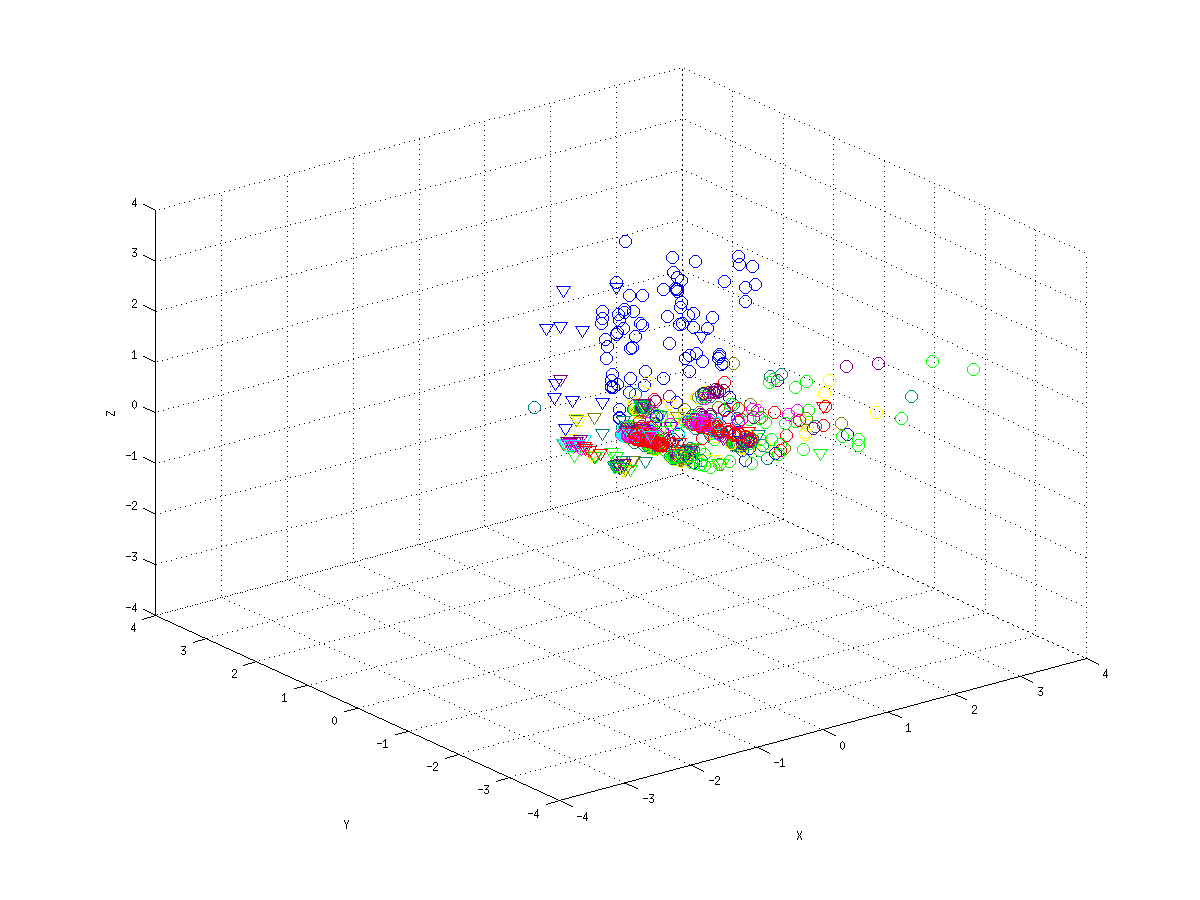
\includegraphics[width=\textwidth]{graficos/fold1_criterioParadap_reglaM_alpha0_rep2_0P.png}
                \caption{Vista en perspectiva.}
        \end{subfigure}%
        ~
        \begin{subfigure}[b]{0.49\textwidth}
                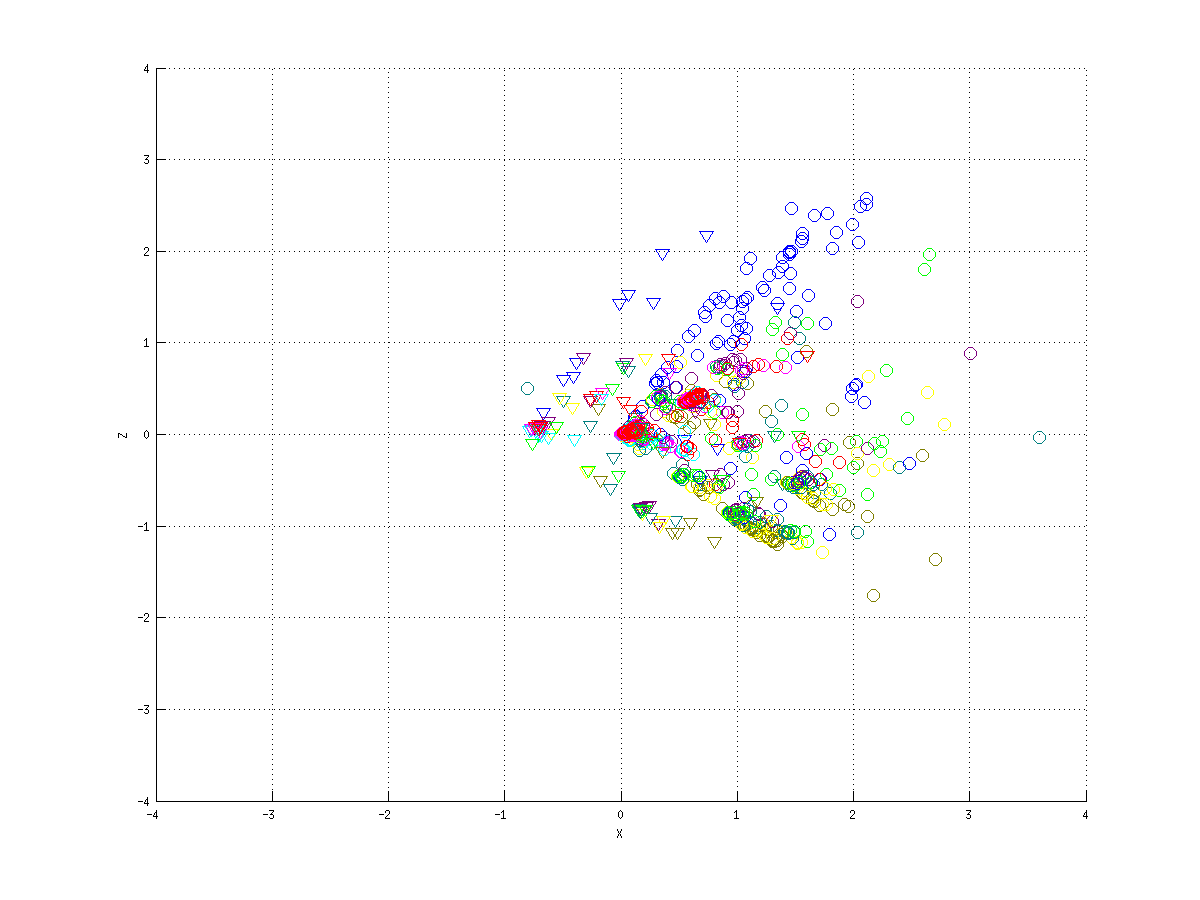
\includegraphics[width=\textwidth]{graficos/fold1_criterioParadap_reglaM_alpha0_rep2_1XZ.png}
                \caption{Plano X-Z.}
        \end{subfigure}
        
        \hspace*{-6.5cm}
        \begin{subfigure}[b]{0.49\textwidth}
                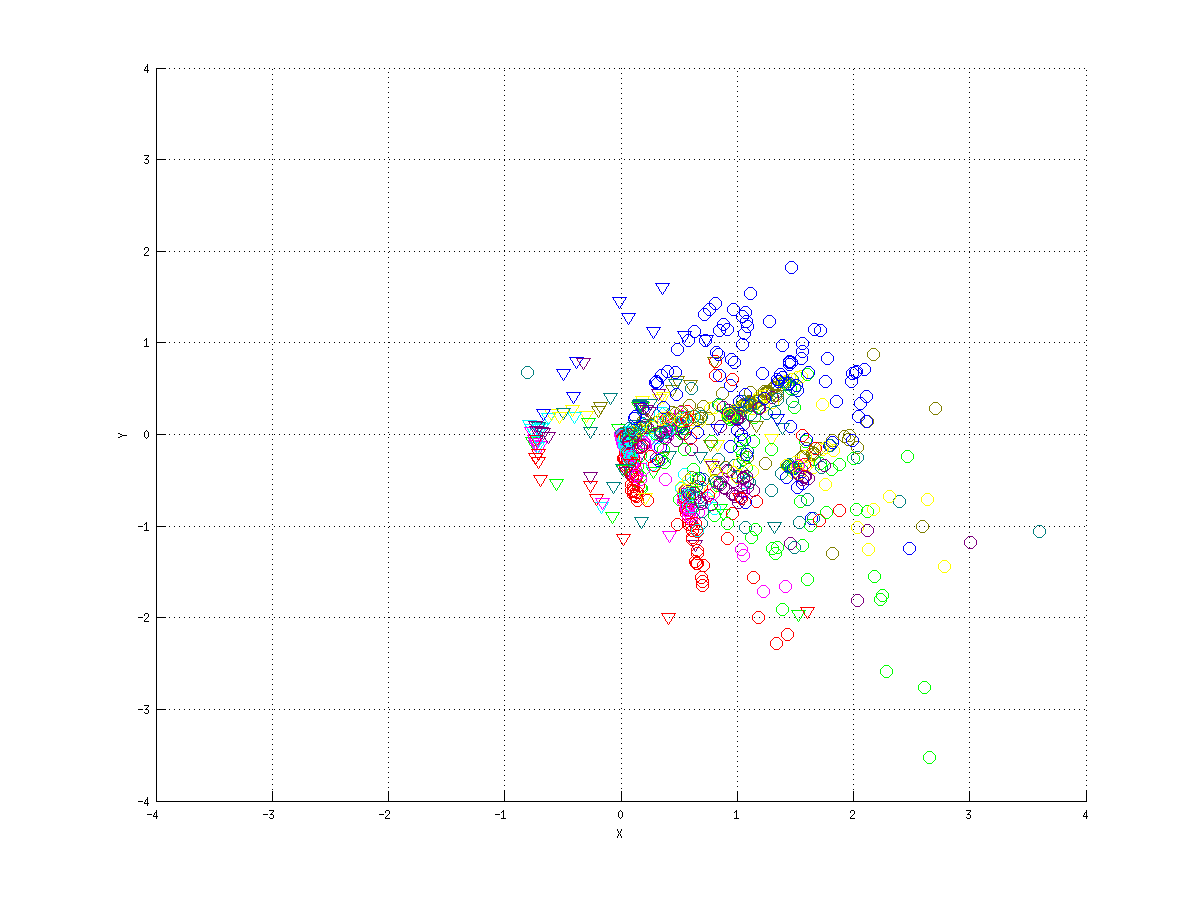
\includegraphics[width=\textwidth]{graficos/fold1_criterioParadap_reglaM_alpha0_rep2_2XY.png}
                \caption{Plano X-Y.}
        \end{subfigure}
        ~
        \begin{subfigure}[b]{0.49\textwidth}
                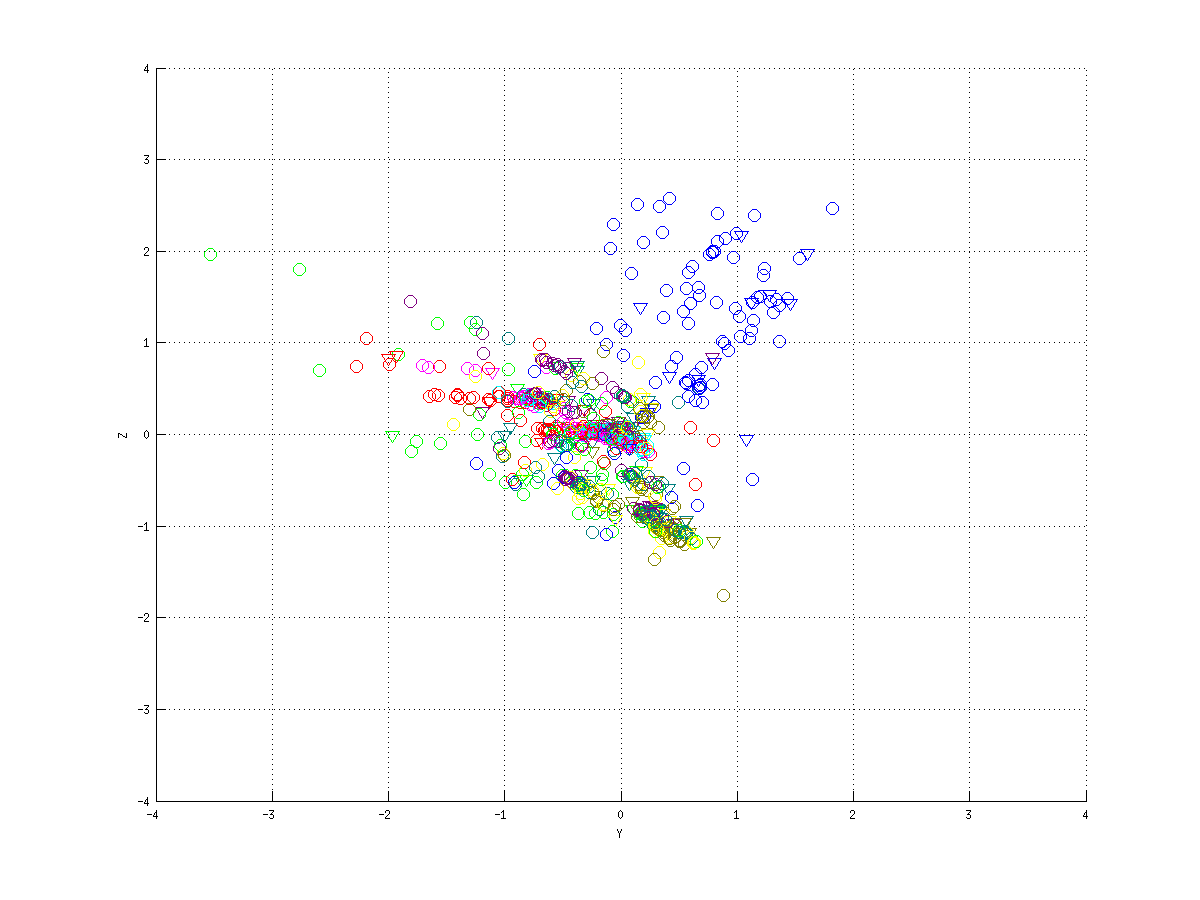
\includegraphics[width=\textwidth]{graficos/fold1_criterioParadap_reglaM_alpha0_rep2_3YZ.png}
                \caption{Plano Y-Z.}
        \end{subfigure}
	\restoregeometry
        \caption{Gráfico espacial para el Fold 1 usando $\Delta W$ como criterio de parada y la regla de Oja con learning rate 0.001 en la repetición 2.}
        \label{fig:fold1_criterioParadap_reglaM_alpha0_rep2}
	\end{figure}
      
      
	\begin{figure}[H]
	\newgeometry{textwidth=21cm,textheight=21cm}
        \centering
        \hspace*{-6.5cm}
        \begin{subfigure}[b]{0.49\textwidth}
                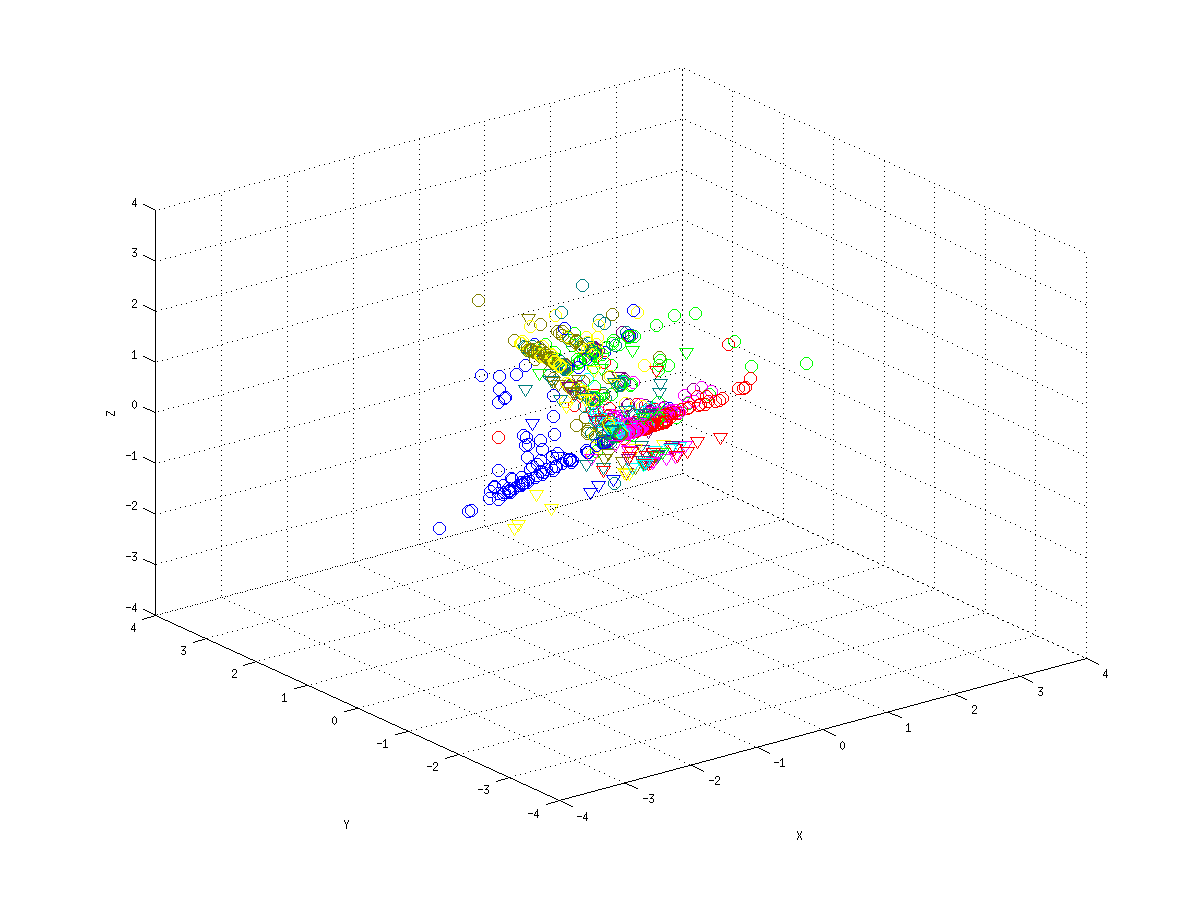
\includegraphics[width=\textwidth]{graficos/fold6_criterioParadap_reglaM_alpha0_rep3_0P.png}
                \caption{Vista en perspectiva.}
        \end{subfigure}%
        ~
        \begin{subfigure}[b]{0.49\textwidth}
                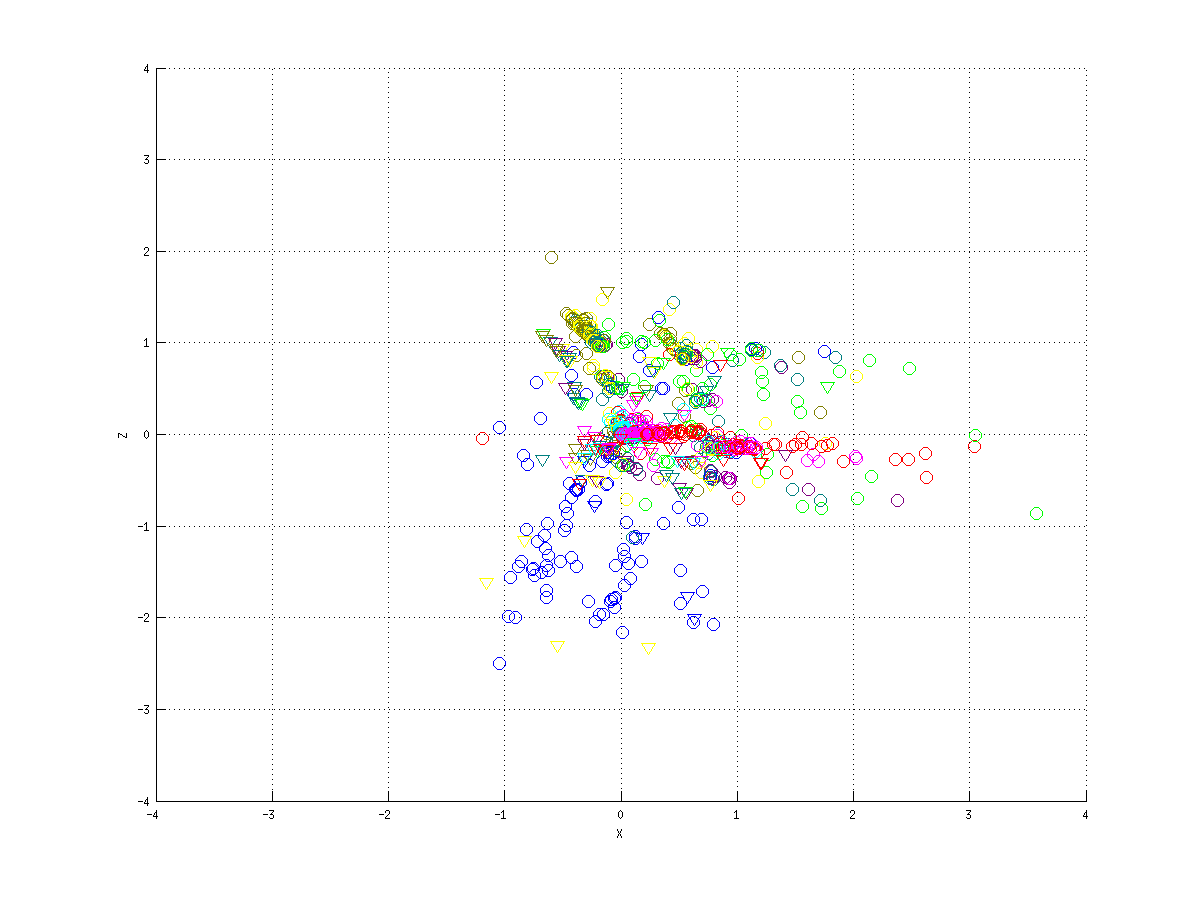
\includegraphics[width=\textwidth]{graficos/fold6_criterioParadap_reglaM_alpha0_rep3_1XZ.png}
                \caption{Plano X-Z.}
        \end{subfigure}
        
        \hspace*{-6.5cm}
        \begin{subfigure}[b]{0.49\textwidth}
                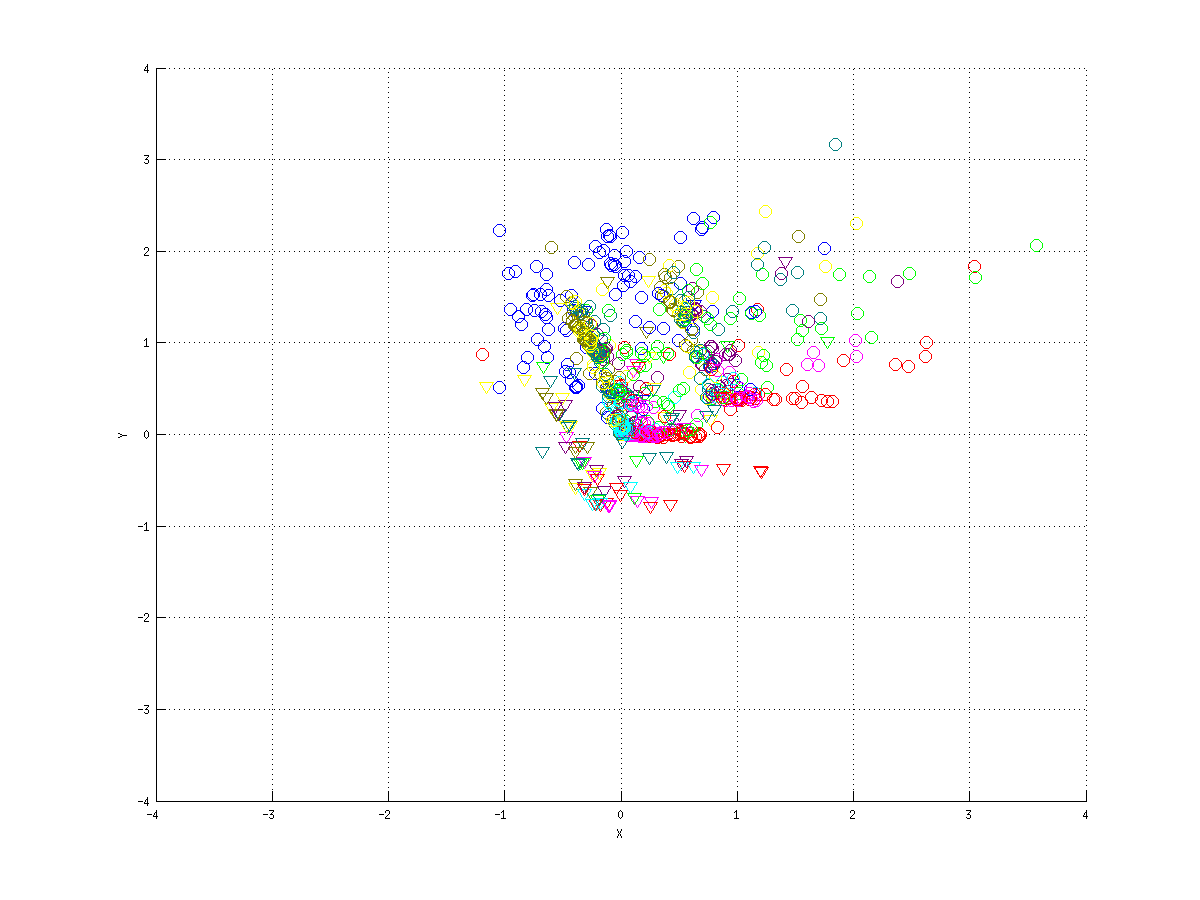
\includegraphics[width=\textwidth]{graficos/fold6_criterioParadap_reglaM_alpha0_rep3_2XY.png}
                \caption{Plano X-Y.}
        \end{subfigure}
        ~
        \begin{subfigure}[b]{0.49\textwidth}
                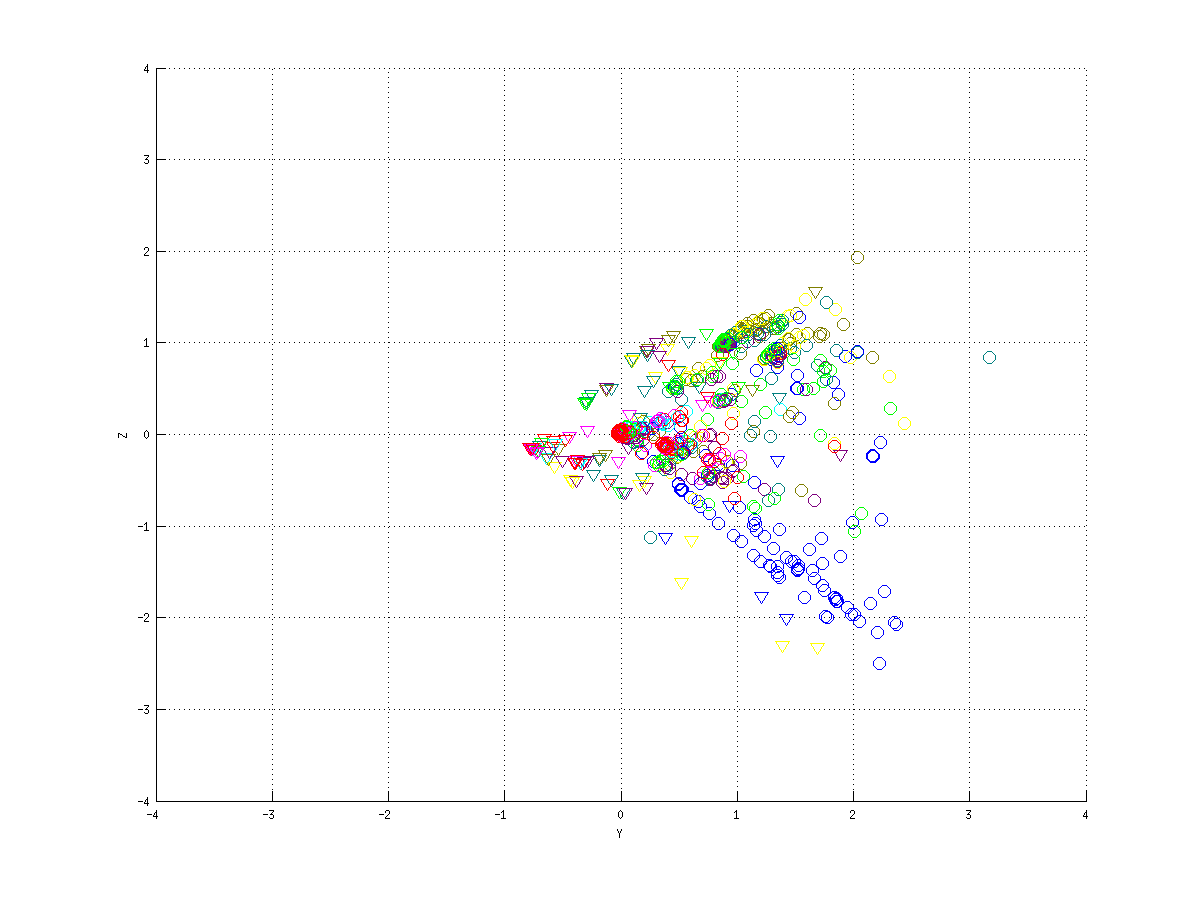
\includegraphics[width=\textwidth]{graficos/fold6_criterioParadap_reglaM_alpha0_rep3_3YZ.png}
                \caption{Plano Y-Z.}
        \end{subfigure}
	\restoregeometry
        \caption{Gráfico espacial para el Fold 6 usando $\Delta W$ como criterio de parada y la regla de Oja con learning rate 0.001 en la repetición 3.}
        \label{fig:fold6_criterioParadap_reglaM_alpha0_rep3}
	\end{figure}
      
      
      
      
      \myparagraph{Particularidades con regla de Sanger y criterio de $\Delta W$}
      
	Los resultados usando la regla de Sanger con el criterio de delta pesos son, tal vez, los más homogéneos en el sentido que todos los gráficos tienen características similares. Como se puede ver en las Figuras \ref{fig:fold1_criterioParadap_reglas_alpha0_rep3} y \ref{fig:fold1_criterioParadap_reglas_alpha0_rep5}, si bien la ubicación espacial cambia, la posiciń relativa entre las instancias de las distintas clases es bastante similar. 
	
	En general, las instancias de la clase azul vuelven a aparecer alejadas del resto como en los casos anteriores. De manera similar las clases roja y celeste ocupan lugares similares y por otro lado lo mismo sucede con las amarilla, marrón y verde. Bajo esta combinación de parámetros sí sucede que la clase magenta aparece más dispersa, algo no tan común en los otros casos. Para el resto de las clases, las dispersiones son similares a casos anteriores ya discutidos.
	
	En este caso sucede también que las instancias de validación se encuentran cerca de las de entrenamiento correspondientes a la misma clase de modo que, al igual que antes, es un buen indicio para una futura clasificación.
 
	\begin{figure}[H]
	\newgeometry{textwidth=21cm,textheight=21cm}
        \centering
        \hspace*{-6.5cm}
        \begin{subfigure}[b]{0.49\textwidth}
                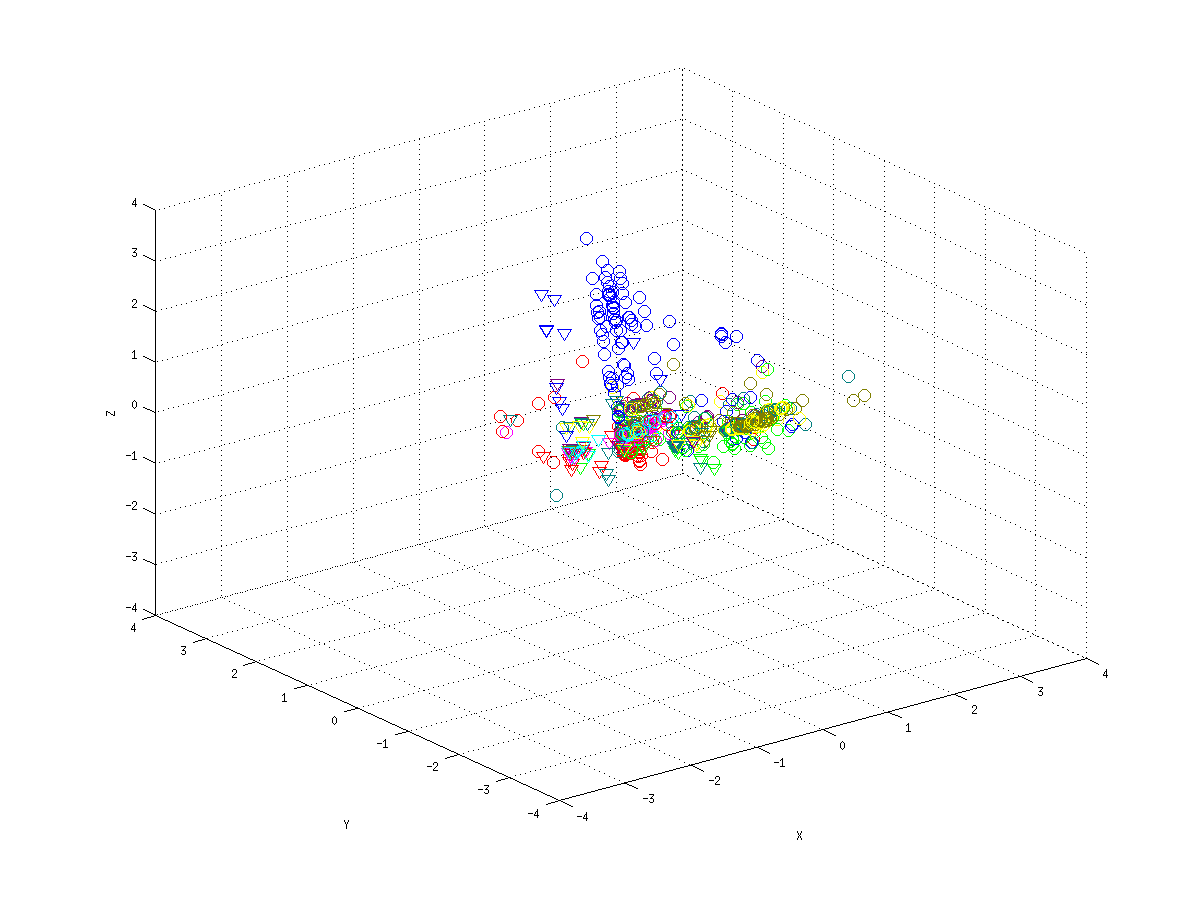
\includegraphics[width=\textwidth]{graficos/fold1_criterioParadap_reglas_alpha0_rep3_0P.png}
                \caption{Vista en perspectiva.}
        \end{subfigure}%
        ~
        \begin{subfigure}[b]{0.49\textwidth}
                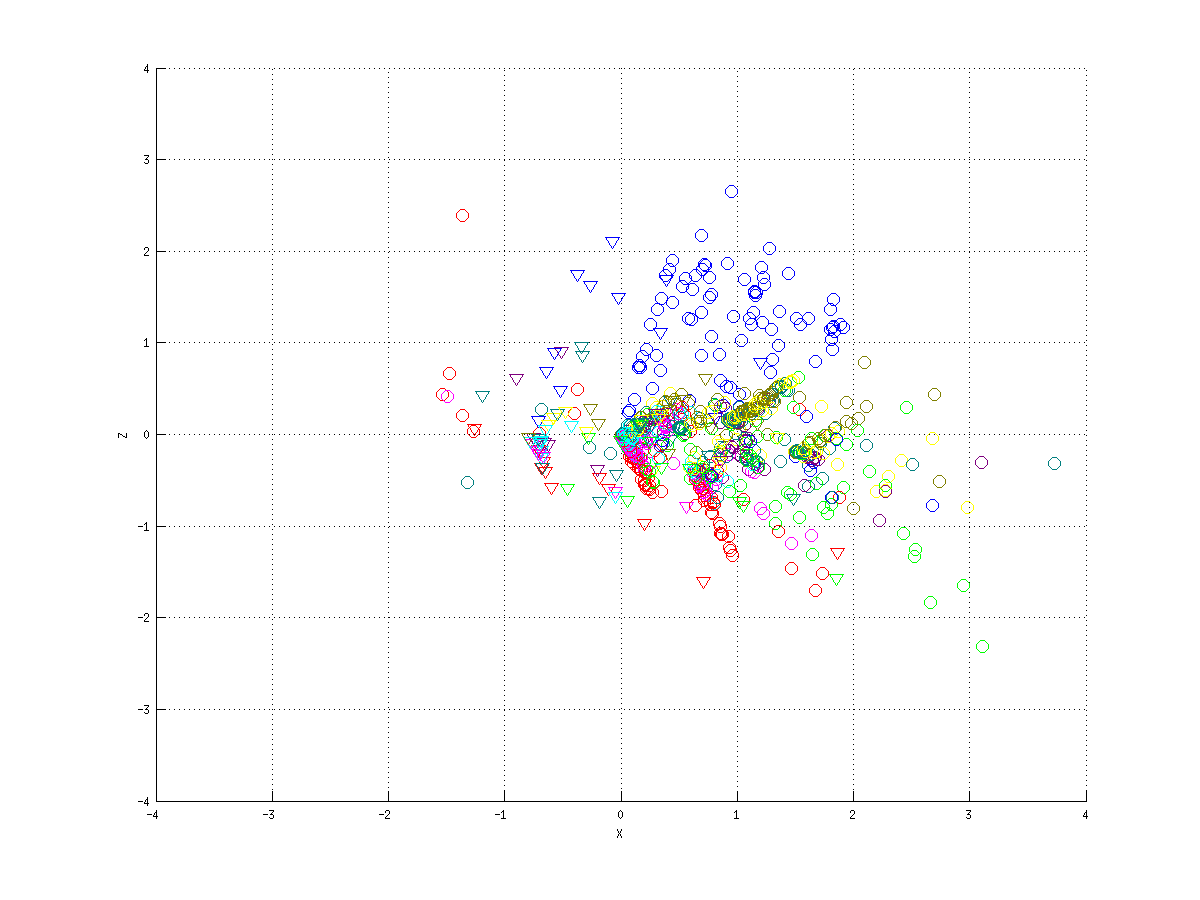
\includegraphics[width=\textwidth]{graficos/fold1_criterioParadap_reglas_alpha0_rep3_1XZ.png}
                \caption{Plano X-Z.}
        \end{subfigure}
        
        \hspace*{-6.5cm}
        \begin{subfigure}[b]{0.49\textwidth}
                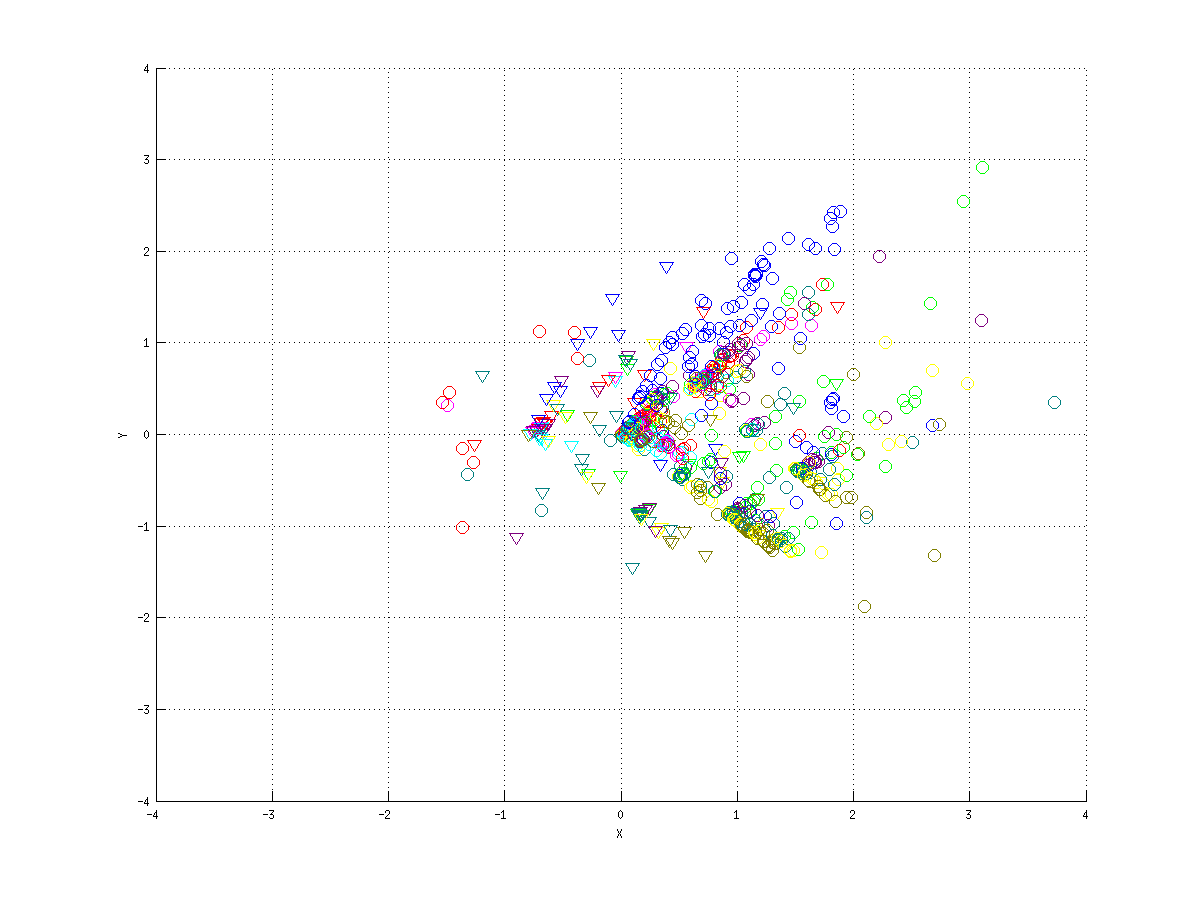
\includegraphics[width=\textwidth]{graficos/fold1_criterioParadap_reglas_alpha0_rep3_2XY.png}
                \caption{Plano X-Y.}
        \end{subfigure}
        ~
        \begin{subfigure}[b]{0.49\textwidth}
                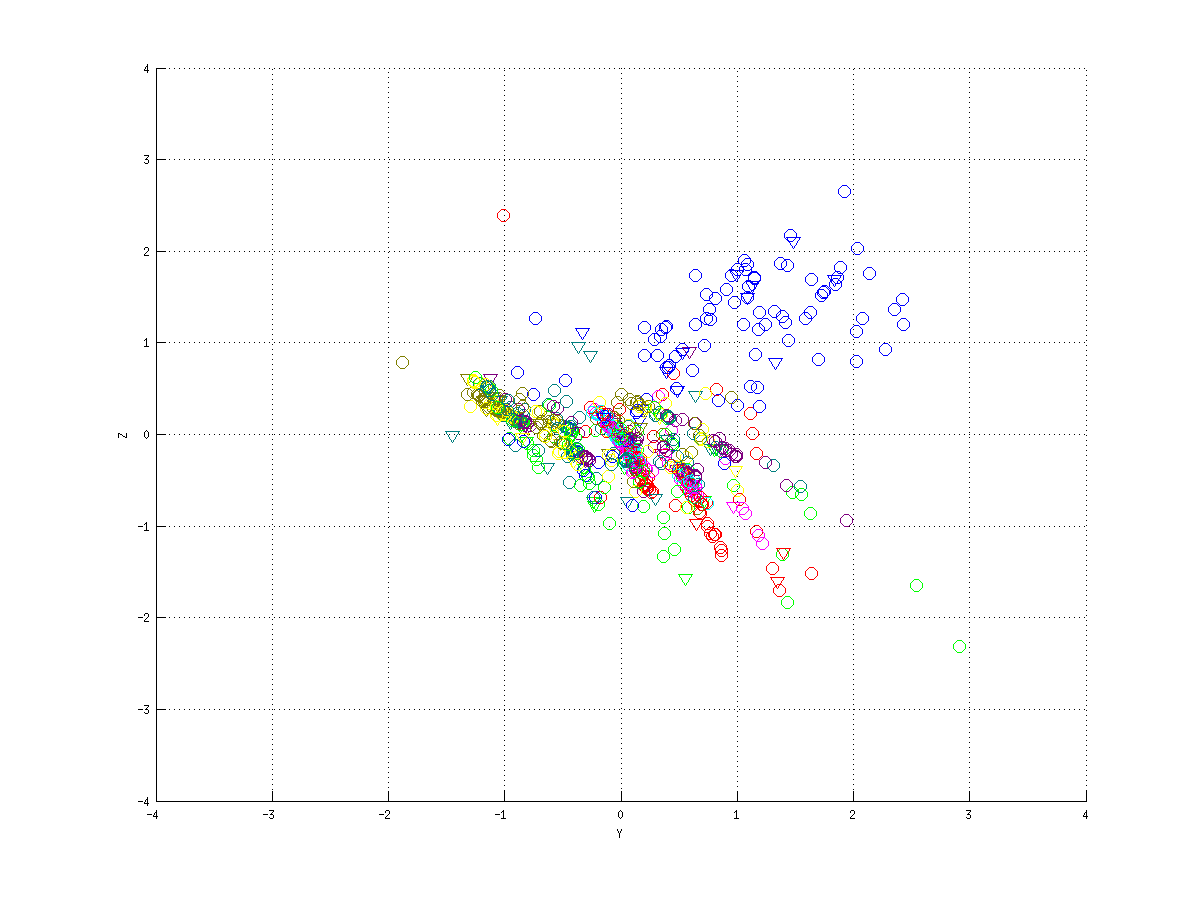
\includegraphics[width=\textwidth]{graficos/fold1_criterioParadap_reglas_alpha0_rep3_3YZ.png}
                \caption{Plano Y-Z.}
        \end{subfigure}
	\restoregeometry
        \caption{Gráfico espacial para el Fold 1 usando $\Delta W$ como criterio de parada y la regla de Sanger con learning rate 0.001 en la repetición 3.}
        \label{fig:fold1_criterioParadap_reglas_alpha0_rep3}
	\end{figure}
      
      
	\begin{figure}[H]
	\newgeometry{textwidth=21cm,textheight=21cm}
        \centering
        \hspace*{-6.5cm}
        \begin{subfigure}[b]{0.49\textwidth}
                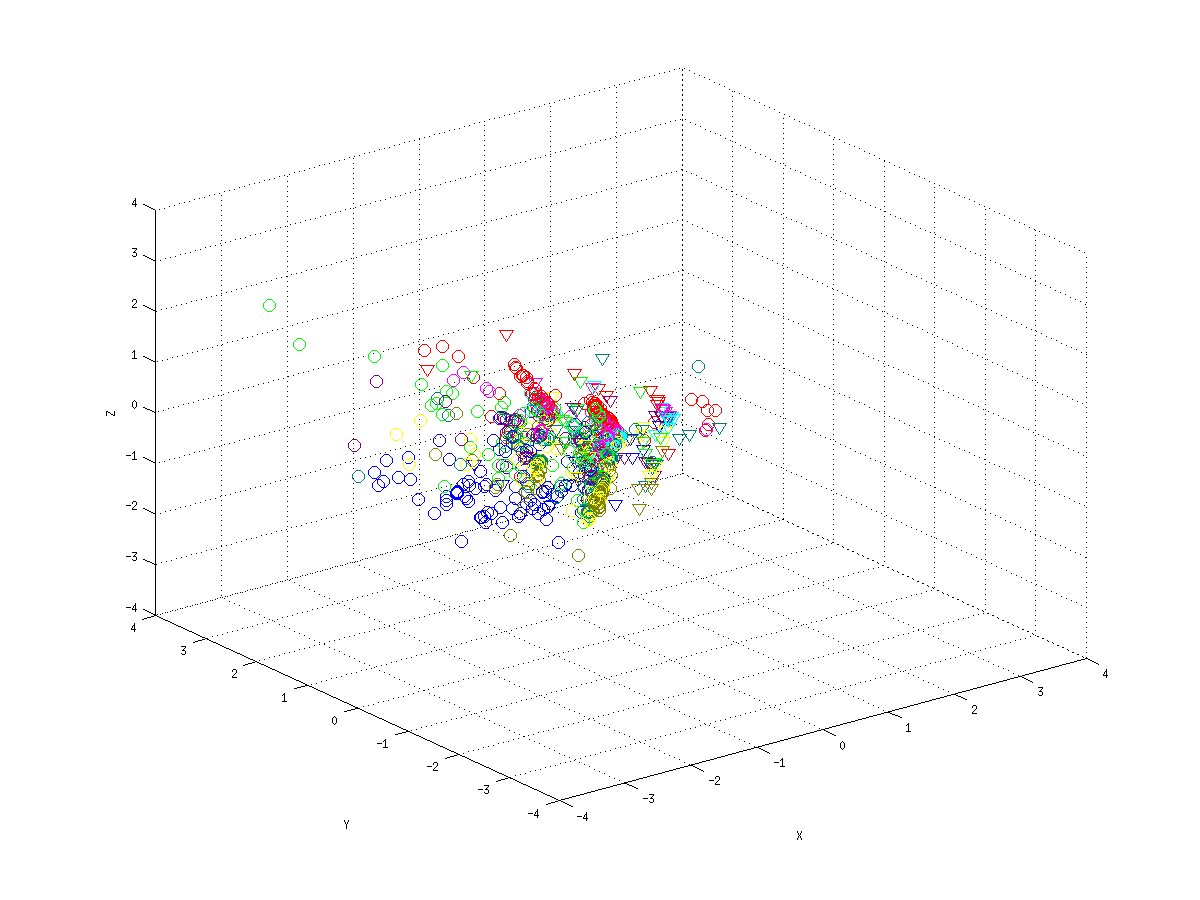
\includegraphics[width=\textwidth]{graficos/fold1_criterioParadap_reglas_alpha0_rep5_0P.png}
                \caption{Vista en perspectiva.}
        \end{subfigure}%
        ~
        \begin{subfigure}[b]{0.49\textwidth}
                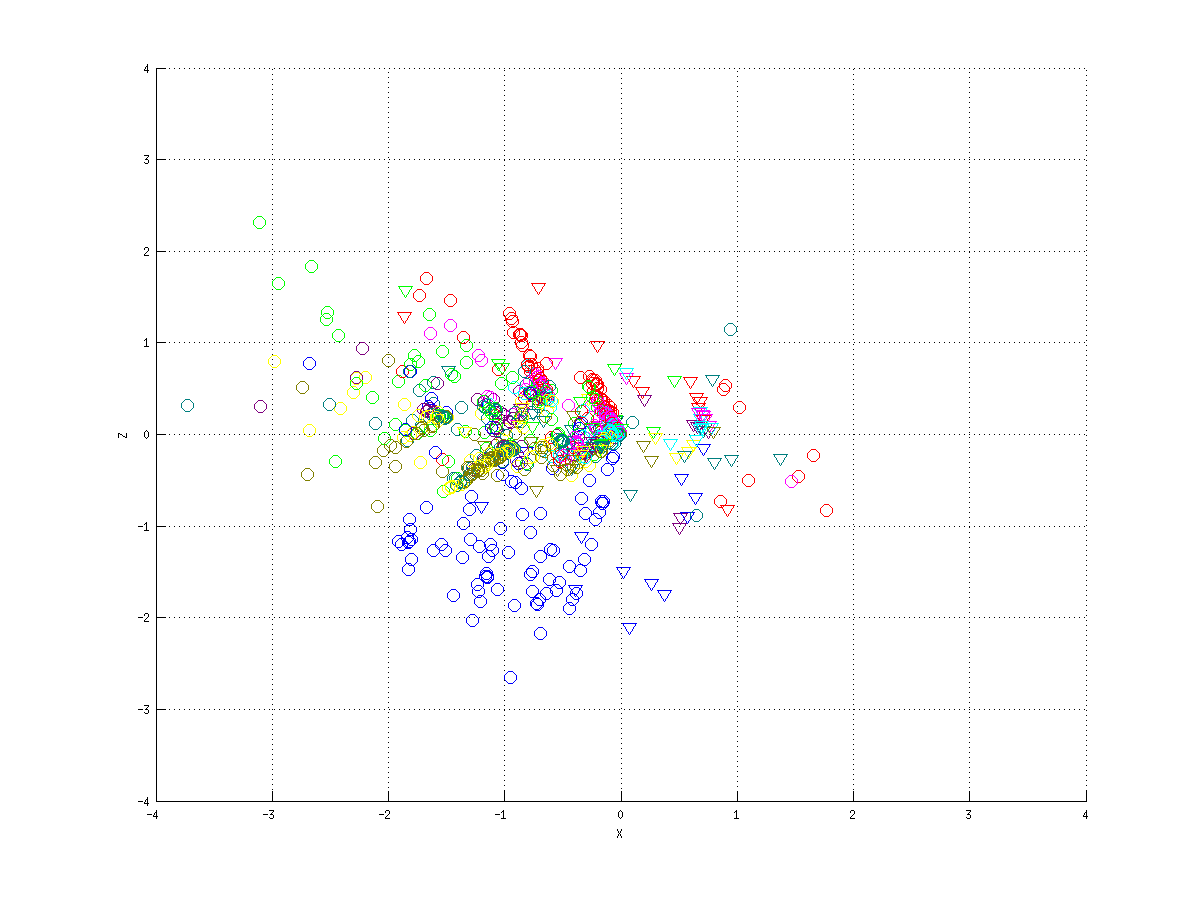
\includegraphics[width=\textwidth]{graficos/fold1_criterioParadap_reglas_alpha0_rep5_1XZ.png}
                \caption{Plano X-Z.}
        \end{subfigure}
        
        \hspace*{-6.5cm}
        \begin{subfigure}[b]{0.49\textwidth}
                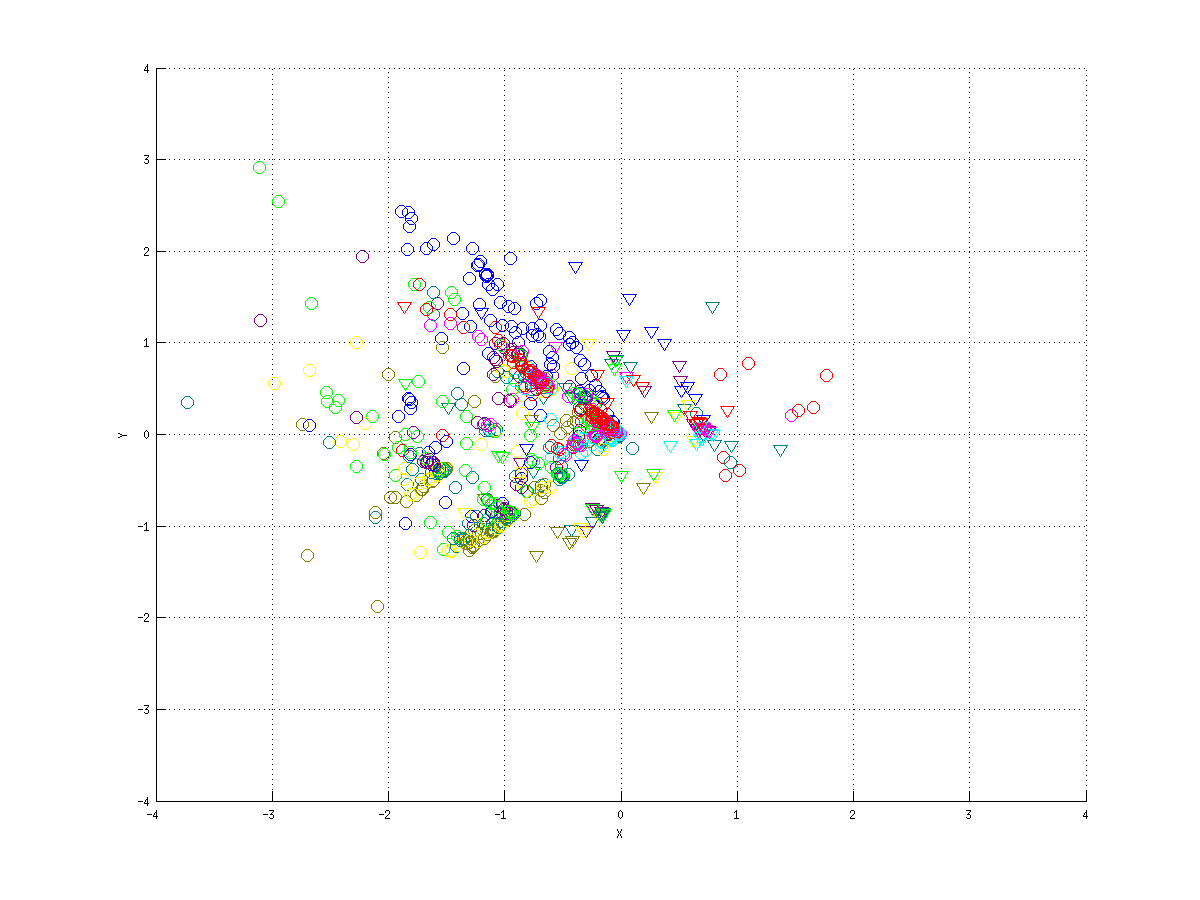
\includegraphics[width=\textwidth]{graficos/fold1_criterioParadap_reglas_alpha0_rep5_2XY.png}
                \caption{Plano X-Y.}
        \end{subfigure}
        ~
        \begin{subfigure}[b]{0.49\textwidth}
                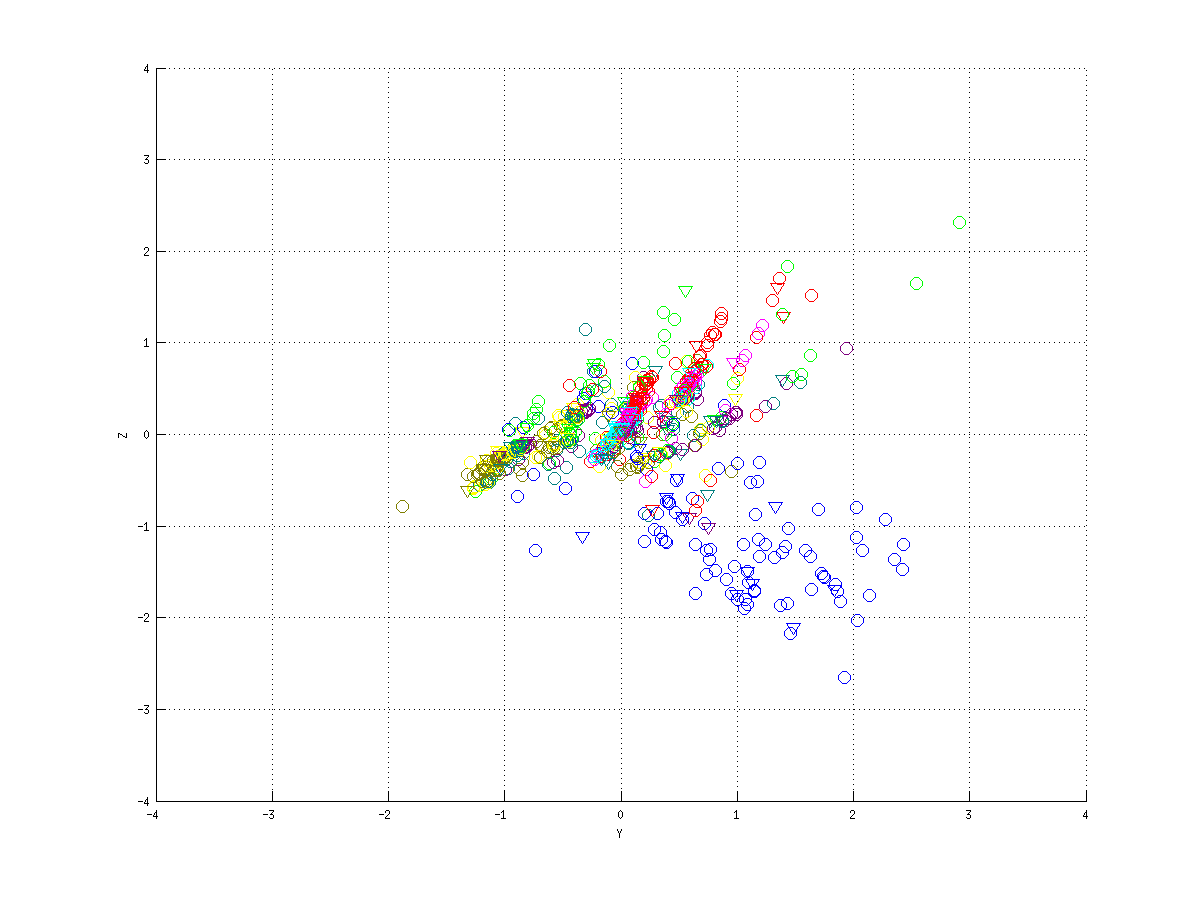
\includegraphics[width=\textwidth]{graficos/fold1_criterioParadap_reglas_alpha0_rep5_3YZ.png}
                \caption{Plano Y-Z.}
        \end{subfigure}
	\restoregeometry
        \caption{Gráfico espacial para el Fold 1 usando $\Delta W$ como criterio de parada y la regla de Sanger con learning rate 0.001 en la repetición 5.}
        \label{fig:fold1_criterioParadap_reglas_alpha0_rep5}
	\end{figure} 
 
 
 
      Dados los resultados obtenidos en la experimentación y considerando que en general se obtuvieron los m\'aximos niveles de convergencia (dado que espacialmente los resultados con el m\'aximo de \'epocas fueron similares a cuando se cort\'o por el criterio, ya sea por pesos o por ortogonalidad), decidimos analizar la velocidad de convergencia al usar un m\'etodo adaptativo. 
 
      Para ello utilizamos diferentes funciones para modificar el learning rate, sin embargo, los resultados obtenidos no fueron buenos. En todos los casos, o bien el algoritmo alcanzó los criterios de convergencia (ortogonalidad o pesos) con una \'epoca arrojando resultados incorrectos o bien el learning rate no permit\'ia la convergencia y acab\'abamos obteniendo valores Not a Number en la matriz de pesos. En el primer caso consideramos que se debe a que ante la primera época, luego de actualizar el learning rate los pesos se modifican de modo que satisfacen trivialmente los criterios. En el segundo caso se debe a que el learning rate es demasiado grande y hace que la matriz de pesos aumente y dada la realimentación positiva por los valores de los pesos entonces al actualizarlos éstos crezcan cada vez más.
      
      Las opciones consideradas fueron:
      
      \begin{itemize}
	\item $\eta = epoca ^ {-\frac{1}{2}}$
	\item $\eta = \alpha ^ {-epoca}$
	\item $\eta = epoca ^ {-\alpha}$
      \end{itemize}
      
      donde $\alpha$ fue un parámetro variado en valores mayores y menores a 1 y $epoca$ es la época actual.

 
      
    \subsection{Mapeo de características}
    
      En este caso, el analisis de este modelo se vuelve algo particular. Para realizar el mismo, decidimos utilizar dos metricas: la primera con el objetivo de obtener alguna nocion de desempe\~no de la red, y la segunda para conocer que tan distanciados estaban los distintos grupos de activacion luego del entrenamiento.
      
      \subsubsection{Distancia a dominantes (DD)}
      
      Representar\'a la distancia relativa media entre los dominantes del set de validaci\'on y el set de activaci\'on. Para generar su calculo, tomamos cada uno de los dominantes del mapa de validacion y buscamos el dominante mas cercano en el mapa de entrenamiento, en el mejor caso esta distancia es cero. 
      
      ~
      
      Obteniendo todas las distancias entre los distintos dominantes calcularemos su media y luego la normalizaremos diviendola por la distancia maxima que puede existir; esto es $||(M_1,M_2)||$, es decir la distancia entre las esquinas de la matriz de pesos.
      
      $$DD(DTr, DTe, W, M_1, M_2) = \frac{dM(mAct(DTr,W), mAct(DTe,W))}{||(M_1,M_2)||}$$
      
      Donde $DTr$ es el dataset de entrenamiento, $DTe$ es el dataset de validacion, $W$ es la matriz de pesos y $M_1, M_2$  son las dimensiones de la ultima. Se supone que $mAct$ calcula los mapas de dominantes para los datos otorgados y que $dM$ calcula la distancia media entre dichos dominantes.
      
      \subsubsection{Factor de cruce (FC)}
      
      Esta metrica nos dara una nocion de cuantas neuronas se activan mas de una clase. Esto nos sirve para observar de que forma la red neuronal esta respondiendo a distintos impulsos. Inferimos que es deseable que este factor sea bajo, ya que lo ideal seria que las distintas clases activen grupos de neuronas disjuntas.
      
      ~
      
      Para calcular este factor, nos armaremos un mapa de la red neuronal en donde tendremos registradas las cantidades de veces que se activo una neurona en las 9 clases distintas. En un escenario ideal, ningun numero deberia ser mayor a 1, ya que indicaria que una neurona se activo para mas de una clase.
      
      ~
      
      Una vez calculado este mapa sumaremos todos los valores de la matriz, le restaremos la cantidad de neuronas que no eran cero dentro del mapa (por lo que en el caso ideal el factor nos daria cero) y lo dividiremos por esa misma cantidad.
      
      $$FD(D, W) = \frac{sumActCruz(D, W) - noSonCero(D, W)}{noSonCero(D, W)}$$
      
      Donde $D$ representa los datos a utilizar y $W$ la matriz de pesos de la red neuronal ya entrenada. Se supone que $sumActCruz$ internamente calcula las activaciones, al igual que $noSonCero$ calcula la cantidad de neuronas que se activaron.
      
      ~
      \subsubsection{Analisis de resultados}
      Para analizar los resultados de las metricas decidimos generar 9 folds distintos para luego promediar los resultados de los mismos. Cada fold tendra un set de entrenamiento y uno de validación generados al azar.
    
      %Para realizar el modelo se consideraron distintos tamaños de mapa así como también la opción de tener parámetros de aprendizaje autoajustables. El objetivo es tener un criterio comparativo para determinar qué tamaño es suficiente en relación a la cantidad de parámetros de las instancias.
      
      %Por otro lado, una vez generados los mapas con el conjunto de entrenamiento, el objetivo es catalogar las instancias del conjunto de validación usando los pesos y el mapa entrenados. 
      

\end{document}